\documentclass[english,10pt]{beamer}

\usetheme[secheader]{Madrid}
\usecolortheme{beaver}
\setbeamertemplate{navigation symbols}{}
\setbeamertemplate{footline}[frame number]
\setbeamertemplate{blocks}[rounded][shadow=true]
\setbeamersize{text margin left=1.2em, text margin right=1.2em}

\usepackage[english]{babel}
\usepackage[utf8]{inputenc}
\usepackage[T1]{fontenc}
\usepackage{lmodern}
\usepackage{amsmath,amssymb}
\usepackage{graphicx}
\usepackage{booktabs}
\usepackage{multirow}
\usepackage{siunitx}
\usepackage{hyperref}
\usepackage{subfig}
\usepackage{tikz}
\usepackage{caption}
\usepackage{xcolor}
\definecolor{darkblue}{RGB}{16,55,110}
\definecolor{unired}{RGB}{200,40,40}

\setbeamercolor{title}{fg=unired}
\setbeamercolor{frametitle}{fg=darkblue}
\setbeamercolor{structure}{fg=darkblue}
\setbeamercolor{block title}{bg=darkblue,fg=white}
\setbeamercolor{block body}{bg=gray!10}

\newcommand{\upgreen}{\textcolor{green!50!black}{$\blacktriangle$}}
\newcommand{\downred}{\textcolor{red}{$\blacktriangledown$}}

\title[CI -- Deblur \& Denoise LBC]{\textbf{Computational Imaging}\\Deblur and Denoise of\\Cervical LBC Cytology Images}
\subtitle{Project -- Group R}
\author[Castaldi, Fusco]{\textbf{Francesco Castaldi}\; \textcolor{gray}{|}\; \textbf{Paolo Fusco}}
\institute[DISI -- UniBO]{Department of Computer Science -- Science and Engineering\\University of Bologna}
\date{A.Y. 2025/2026}
\titlegraphic{
\includegraphics[width=0.22\textwidth]{figures/unibo_logo.png}}
\logo{
\includegraphics[width=0.05\textwidth]{figures/unibo_logo.png}}

\begin{document}

\begin{frame}[plain]
  \titlepage
  \vspace{-0.5cm}
  \begin{center}
    \small\href{https://github.com/FrancescoCastaldi/ci-cervical-lbc}{github.com/FrancescoCastaldi/ci-cervical-lbc}
  \end{center}
\end{frame}

\section{Project Description}

\begin{frame}{Inverse Problem}
  \begin{block}{The problem we face}
    Given a cervical cytology image degraded by \textbf{Gaussian blur} and \textbf{AWGN noise}, we want to estimate the original image.
  \end{block}
  \begin{equation*}
    y = \mathcal{H}(x) + n
  \end{equation*}
  \noindent where $x$ is the original (unknown), $\mathcal{H}$ is the blur ($\sigma=2$, kernel $9\times9$), $n$ is AWGN with $\sigma_n \in \{0.005, 0.01, 0.05, 0.1\}$.
  \vspace{0.15cm}
  \begin{alertblock}{Why it is difficult}
    The problem is \textbf{ill-posed}: infinitely many images $x$ produce the same $y$. A \textbf{prior} is needed: TV encodes it as mathematical regularization, UNet learns it from data, DiffPIR generates it with a diffusion model.
  \end{alertblock}
\end{frame}

\begin{frame}{Selected Methods}
  \begin{center}\small 3 out of 4 methods (excluded Weighted TV)\end{center}
  \vspace{0.2cm}
  \noindent We selected three fundamentally different approaches, one for each methodological family of the course. This allows a comparison that is not only numerical, but also qualitative on the different resolution philosophies.
  \vspace{0.2cm}
  \begin{columns}[t]
    \column{0.33\textwidth}
      \begin{block}{Variational}
        \centering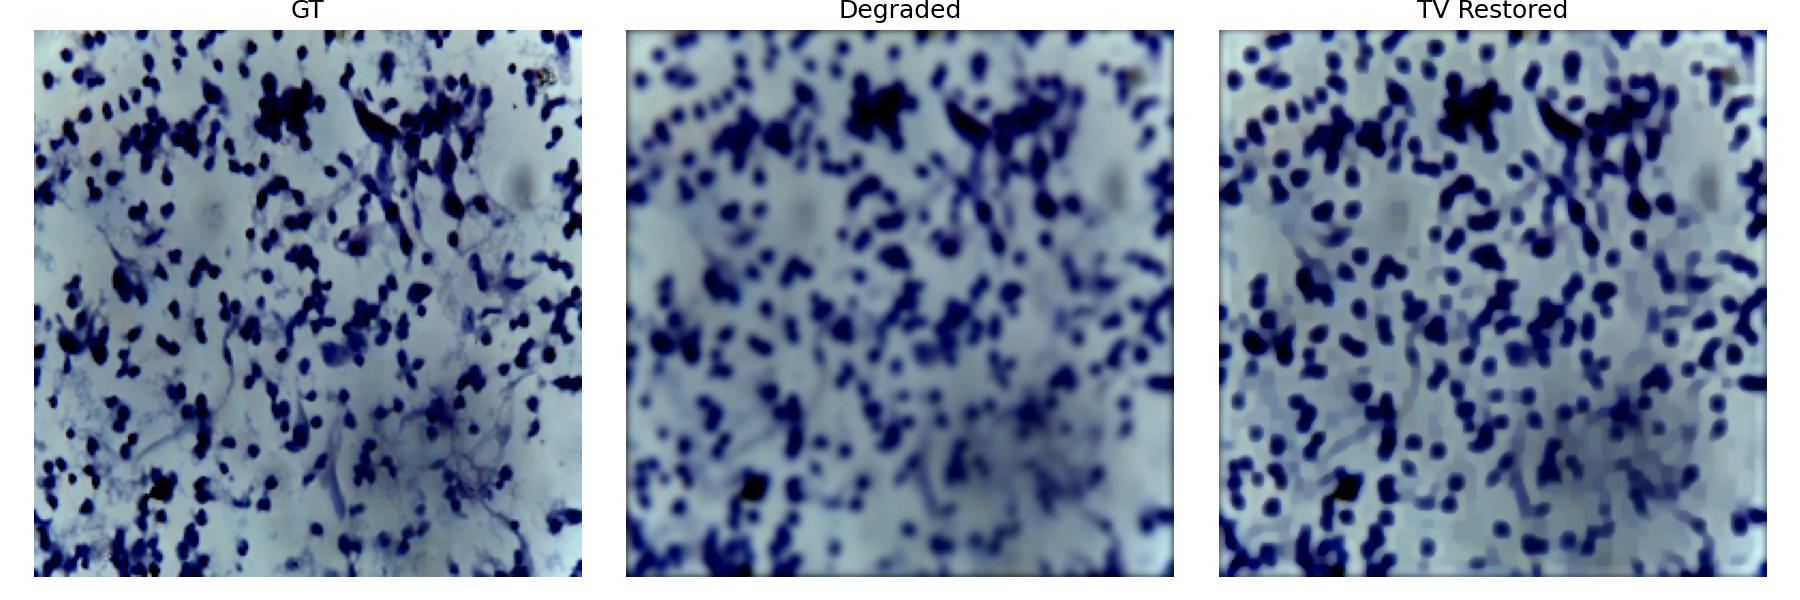
\includegraphics[height=1.1cm]{../results/tv/qualitative/noise_0.005_sample0.png}\\[0.05cm]
        \textbf{Total Variation}
        \begin{itemize}\small
          \item $\lambda=0.005$, Adam, 150 iter
        \end{itemize}
      \end{block}
    \column{0.33\textwidth}
      \begin{block}{Deep Learning}
        \centering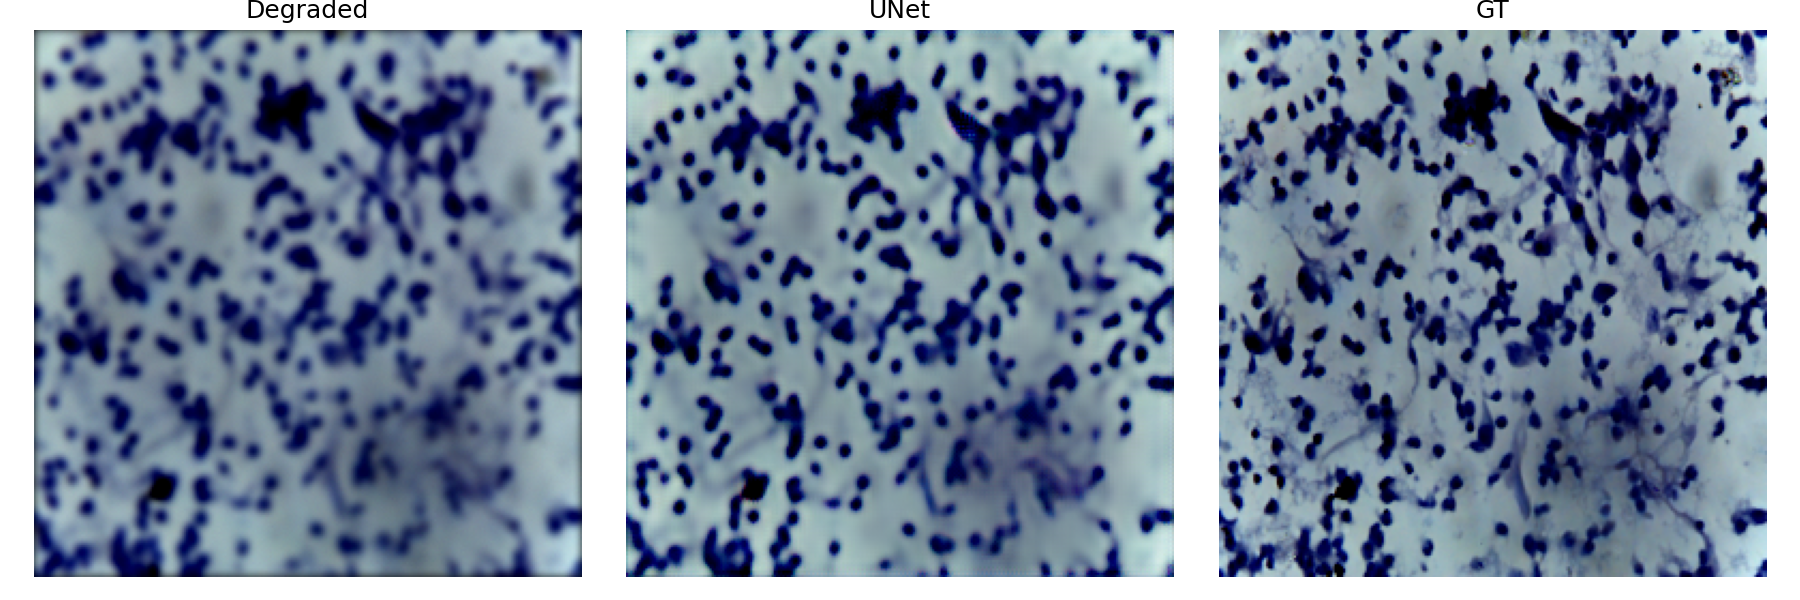
\includegraphics[height=1.1cm]{../results/unet/qualitative/noise_0.005_sample0.png}\\[0.05cm]
        \textbf{UNet}
        \begin{itemize}\small
          \item Encoder-Decoder, L1+Adam
        \end{itemize}
      \end{block}
    \column{0.33\textwidth}
      \begin{block}{Generative}
        \centering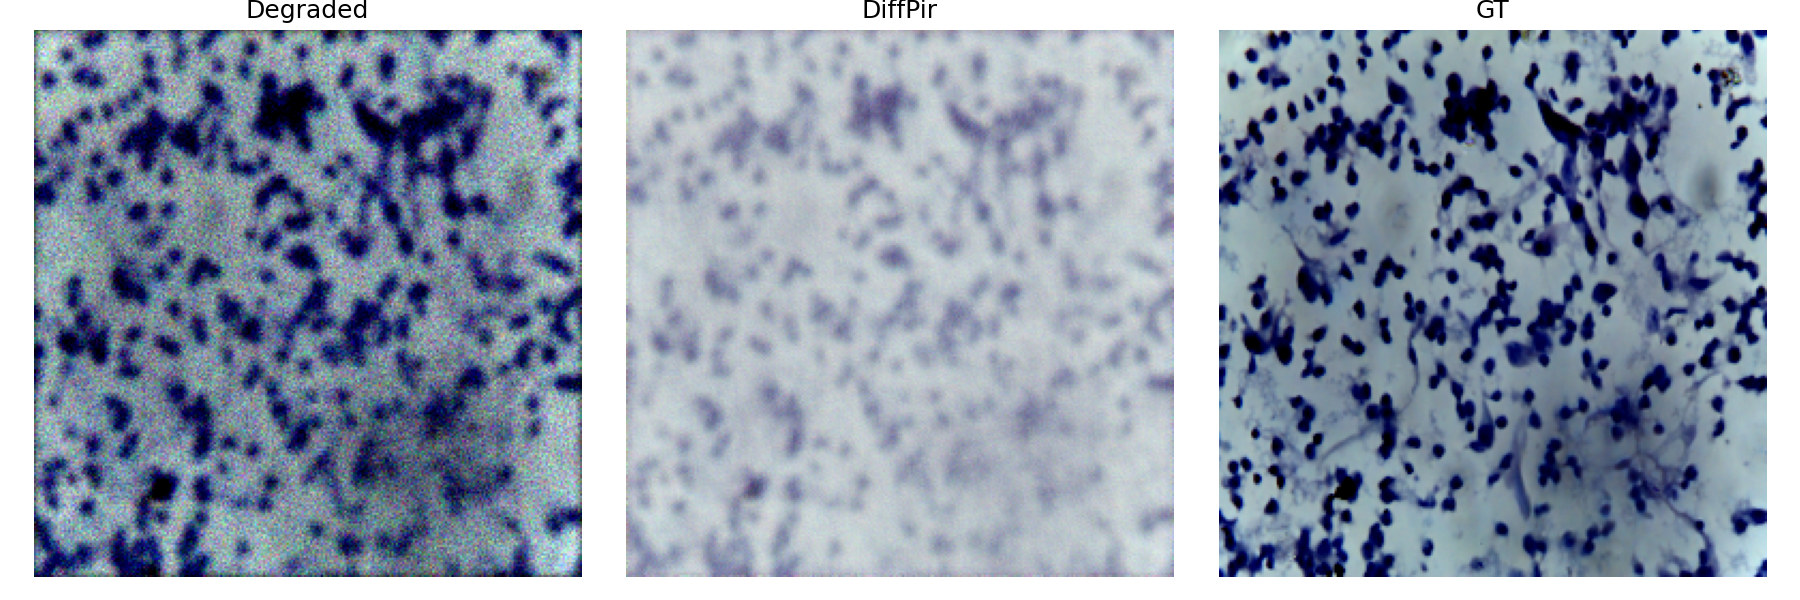
\includegraphics[height=1.1cm]{../results/diffpir/qualitative/noise_0.1_sample0.png}\\[0.05cm]
        \textbf{DiffPIR}
        \begin{itemize}\small
          \item DDPM+LightUNet, FFT fidelity
        \end{itemize}
      \end{block}
  \end{columns}
\end{frame}

\section{Dataset}

\begin{frame}{Mendeley LBC Cervical Cancer}
  \begin{columns}[c] % Allinea verticalmente al centro le due colonne
    
    % Colonna di sinistra: Informazioni e Tabella (più stretta per risparmiare spazio)
    \column{0.45\textwidth}
      \footnotesize % Testo compatto ma perfettamente leggibile nelle slide
      \begin{itemize}
        \item \textbf{962 images} of cervical cytology 
        \item Original $2048\times1536$, \textbf{resized} to $256\times256$ 
        \item Normalized to $[-1,1]$ 
      \end{itemize}
      
      \vspace{0.1cm}
      
      \begin{block}{\footnotesize Diagnostic Classes}
        \centering
        \scriptsize % Ottimizza la tabella per farla stare perfettamente nel blocco strettissimo
        \setlength{\tabcolsep}{4pt} % Riduce lo spazio tra le colonne della tabella
        \begin{tabular}{lrc}\toprule
          \textbf{Class} & \textbf{N} & \textbf{\%}\\\midrule 
          NILM & 612 & 63.6\%\\ 
          HSIL & 163 & 16.9\%\\ 
          LSIL & 113 & 11.7\%\\ 
          SCC  & 74  & 7.7\%\\\bottomrule 
        \end{tabular}
      \end{block}

    % Colonna di destra: Immagine quadrata (più larga, occupa il 55% della slide)
    \column{0.55\textwidth}
      \centering
      \includegraphics[width=\textwidth, keepaspectratio]{../data/degraded/examples/eda_samples_per_class.png}
      
  \end{columns}
\end{frame}

\begin{frame}{Preprocessing and Split}
  \begin{block}{Pipeline}
    \begin{tabular}{lll}\toprule
      \textbf{Step} & \textbf{Operation} & \textbf{Output}\\\midrule
      1 & Bilinear resize $2048\to256$ & $256\times256$\\
      2 & ToTensor $[0,255]\to[0,1]$ & float32\\
      3 & Normalization $(x-0.5)/0.5$ & $[-1,1]$\\
      4 & Stratified split 70/15/15 & train/val/test\\\bottomrule
    \end{tabular}
  \end{block}
  \begin{columns}
    \column{0.5\textwidth}
      \begin{block}{Split}
        \begin{tabular}{lrc}\toprule
          \textbf{Split} & \textbf{\%} & \textbf{Images}\\\midrule
          Training  & 70\% & 673\\
          Validation & 15\% & 144\\
          Test      & 15\% & 145\\\bottomrule
        \end{tabular}
      \end{block}
    \column{0.5\textwidth}
      \begin{itemize}
        \item Fixed seed 42
        \item Stratified by class
        \item Same test set for all
      \end{itemize}
  \end{columns}
\end{frame}

\section{Experimental Setup}

\begin{frame}{Degradation}
  \begin{block}{Identical parameters for all methods}
    \begin{columns}
      \column{0.5\textwidth}
        \centering\textbf{Gaussian Blur}\\[0.1cm]
        $\sigma=2$, kernel $9\times9$
      \column{0.5\textwidth}
        \centering\textbf{AWGN}\\[0.1cm]
        $\sigma_n\in\{0.005,0.01,0.05,0.1\}$
    \end{columns}
  \end{block}

  \vspace{0.15cm}
  \centering
  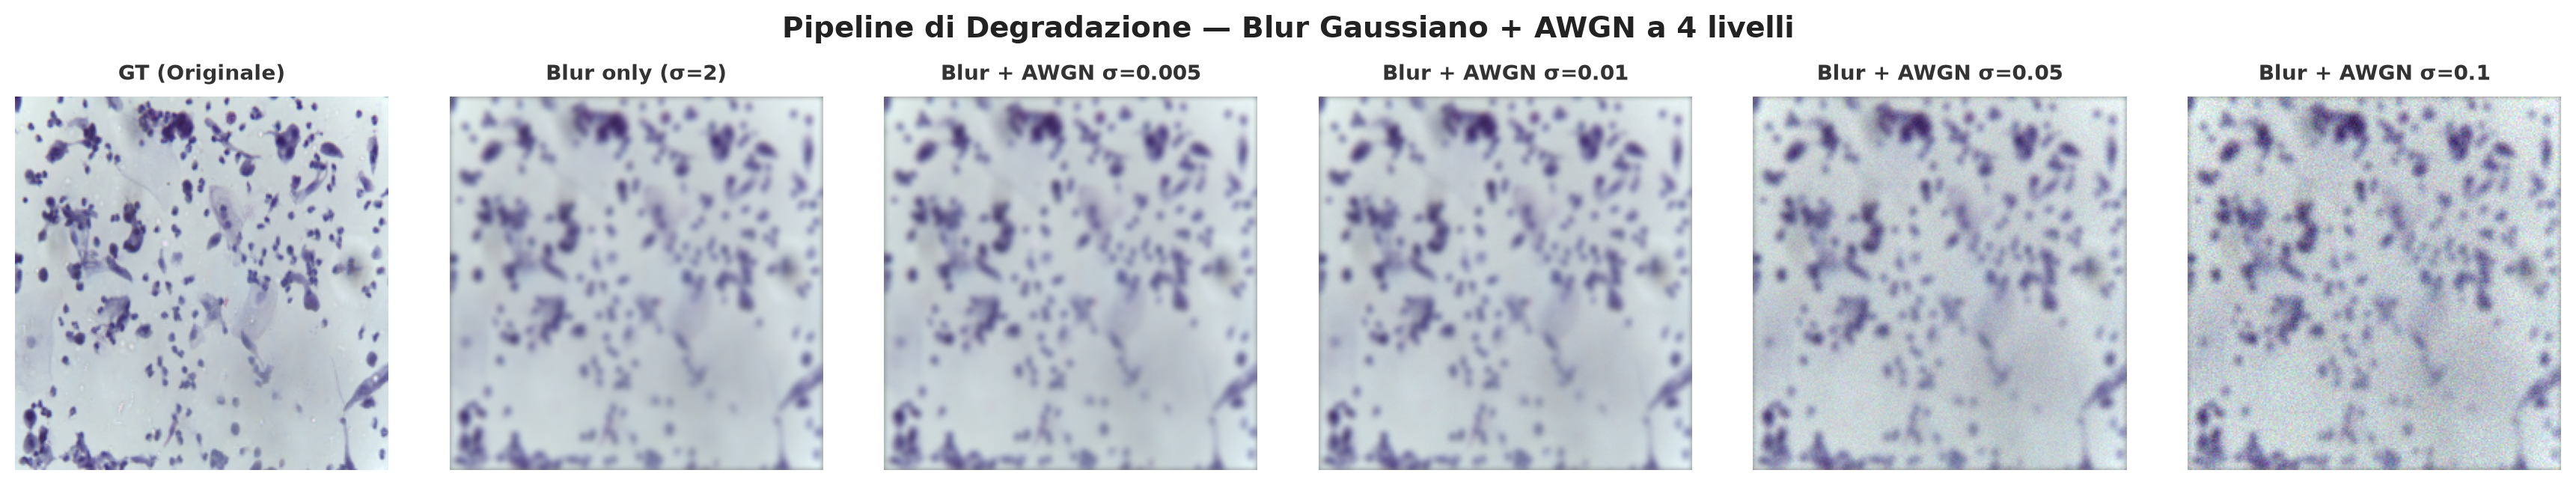
\includegraphics[width=0.95\textwidth]{../results/qualitative_slides/noise_strip_crops.png}

  \vspace{0.15cm}
  \begin{columns}[t]
    \column{0.55\textwidth}\raggedright\small
      \textbf{Pipeline:} blur $H$ on GT $x$ $\to$ add AWGN $n$ ($\sigma_n$) $\to$ clamp $[-1,1]$
      \begin{equation*}
        y = \mathcal{H}(x) + n
      \end{equation*}
    \column{0.4\textwidth}\raggedright\small
      \begin{itemize}
        \item Same pipeline for all methods
        \item Seed 42 for reproducibility
      \end{itemize}
  \end{columns}
\end{frame}

\section{Total Variation}

\begin{frame}{Total Variation -- Theory}
  \begin{block}{Variational model}
    \begin{equation*}
      \hat{x} = \arg\min_x \underbrace{\|H*x - y\|_2^2}_{\text{data fidelity}} + \lambda \cdot \underbrace{TV(x)}_{\text{regularization}}
    \end{equation*}
  \end{block}
  \vspace{0.15cm}
  \noindent The idea is simple: we want an image that, after blur, resembles $y$, but is also \emph{regular}. \textbf{Total Variation} measures regularity: it sums the absolute differences between adjacent pixels.
  \begin{equation*}
    TV(x) = \sum_{i,j} |x_{i+1,j} - x_{i,j}| + |x_{i,j+1} - x_{i,j}|
  \end{equation*}
  \noindent Unlike Tikhonov, TV \textbf{preserves edges}: it penalizes small oscillations (noise) but allows sharp jumps. The cost is the \textit{staircasing} effect if $\lambda$ is too high.
  \vspace{0.15cm}
  \begin{block}{Selected parameters}
    After validation: $\lambda_{reg}=0.005$, Adam optimizer ($lr=0.001$), 150 iterations, clamping $[-1,1]$ after each step.
  \end{block}
\end{frame}

\begin{frame}{Total Variation -- Algorithm}
  \begin{columns}
    \column{0.53\textwidth}
      \textbf{Pseudo-code:}
      \vspace{0.15cm}
      \begin{enumerate}
        \item $x \gets y$, $\lambda \gets 0.005$
        \item Adam optimizer ($lr = 10^{-3}$)
        \item \textbf{for} $i = 1$ \textbf{to} $150$ \textbf{do}
        \item \hspace{0.5cm}$x_{blur} \gets H * x$
        \item \hspace{0.5cm}$\mathcal{L} \gets \|x_{blur} - y\|_2^2 + \lambda \cdot TV(x)$
        \item \hspace{0.5cm}$\nabla_x\mathcal{L} \gets$ backpropagation
        \item \hspace{0.5cm}$x \gets$ AdamStep$(x, \nabla_x\mathcal{L})$
        \item \hspace{0.5cm}$x \gets \text{clamp}(x, -1, 1)$
        \item \textbf{end for}
        \item \textbf{return} $x$
      \end{enumerate}
    \column{0.47\textwidth}
      \small
      \textbf{TV Loss:}
      \begin{equation*}
        TV(x) = \sum_{i,j} |x_{i+1,j} - x_{i,j}| + |x_{i,j+1} - x_{i,j}|
      \end{equation*}
      \vspace{0.2cm}
      \textbf{Optimization loop:}
      \begin{enumerate}
        \item Compute $H*x$ (blur)\\\strut
        \item Loss: fidelity + regularization\\\strut
        \item Backpropagation\\\strut
        \item Adam step\\\strut
        \item Clamp to $[-1,1]$
      \end{enumerate}
      \vspace{0.2cm}
      \textbf{Choice of $\lambda$:}
      \begin{itemize}
        \item $\lambda=0.1$: staircasing
        \item $\lambda=0.001$: residual noise
        \item $\lambda=0.005$: optimal balance
      \end{itemize}
  \end{columns}
\end{frame}

\begin{frame}{Total Variation -- Results}
  \begin{columns}
    \column{0.5\textwidth}
      \textbf{PSNR and SSIM on 145 test images}
      \vspace{0.2cm}
      \begin{tabular}{l|cc}\toprule
        $\sigma_n$ & \textbf{PSNR} & \textbf{SSIM}\\\midrule
        0.005 & \textbf{32.09} & \textbf{0.911}\\
        0.01  & \textbf{32.04} & \textbf{0.909}\\
        0.05  & 30.42 & 0.837\\
        0.1   & 26.54 & 0.586\\\bottomrule
      \end{tabular}
      \vspace{0.3cm}
      \begin{itemize}
        \item Excellent at low noise (PSNR $>$ 32 dB)
        \item Progressive degradation with noise
        \item Staircasing visible at $\sigma_n=0.1$
      \end{itemize}
    \column{0.5\textwidth}
      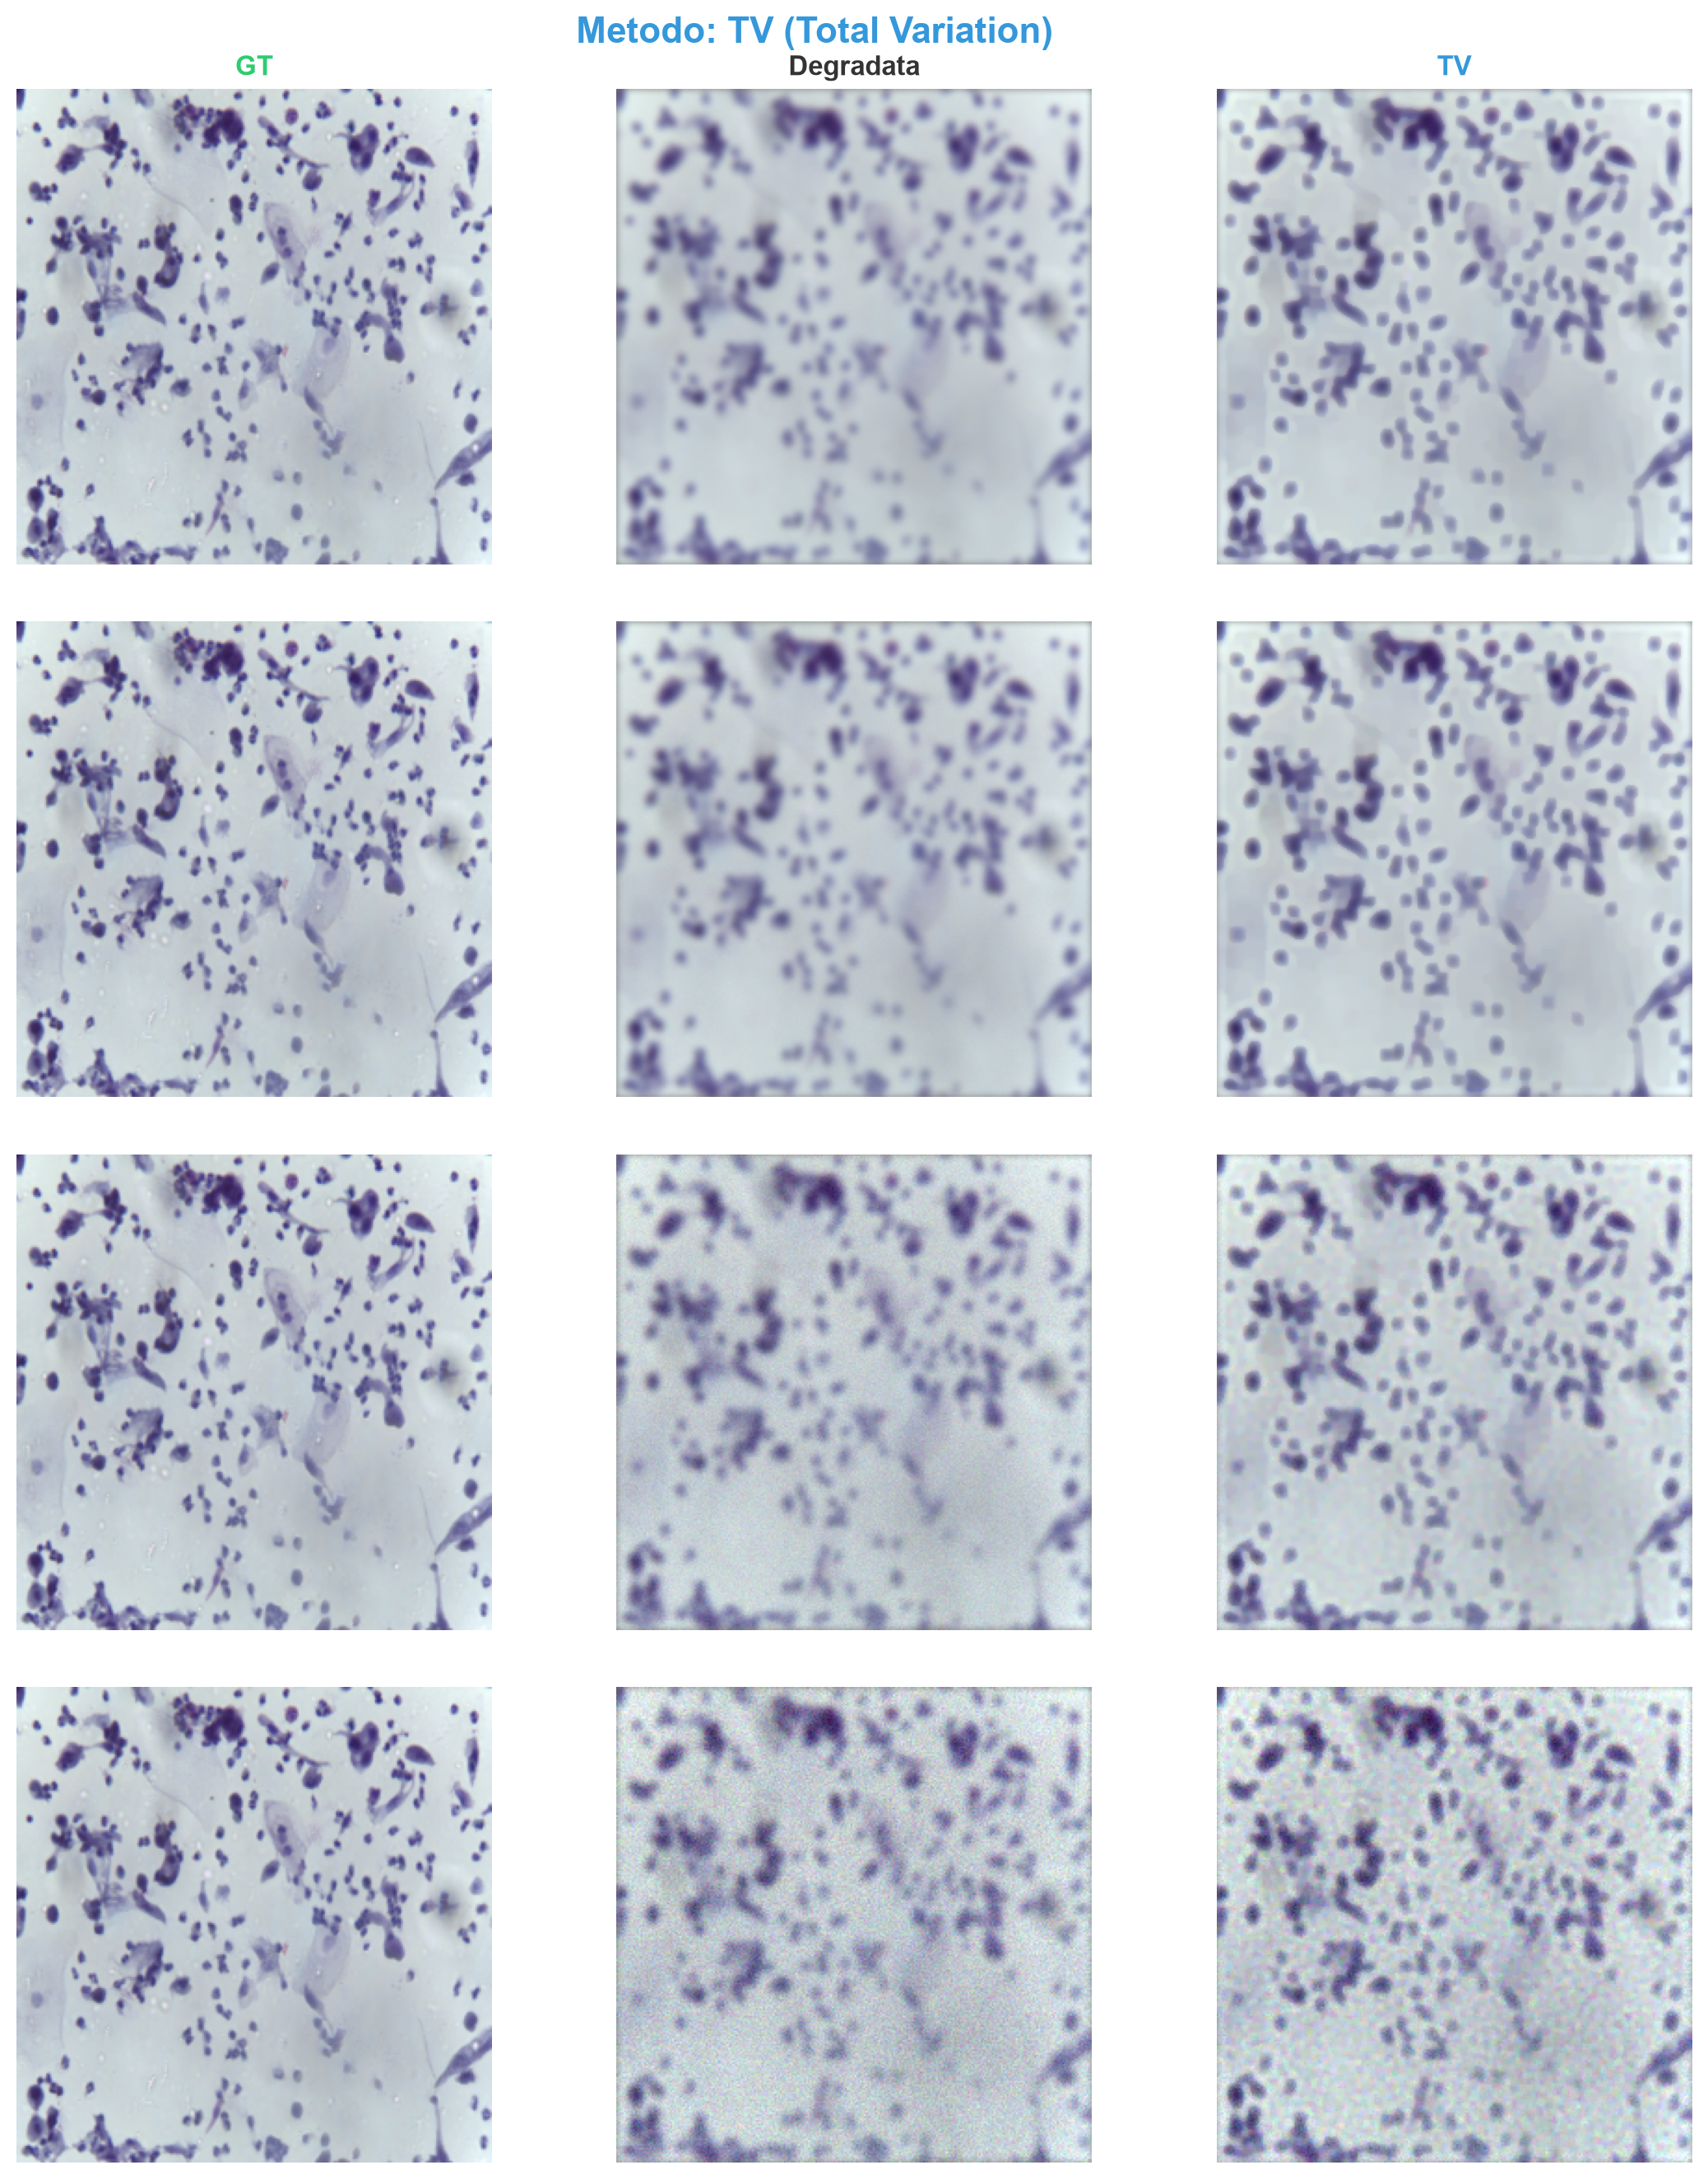
\includegraphics[width=\textwidth]{../results/qualitative_slides/tv_comparison.png}
  \end{columns}
\end{frame}

\section{UNet}

\begin{frame}{UNet -- Architecture}
  \begin{block}{Encoder-Decoder with Skip Connections}
    Lightweight architecture for image-to-image: degraded $\to$ restored
  \end{block}
  \vspace{0.2cm}
  \begin{center}
    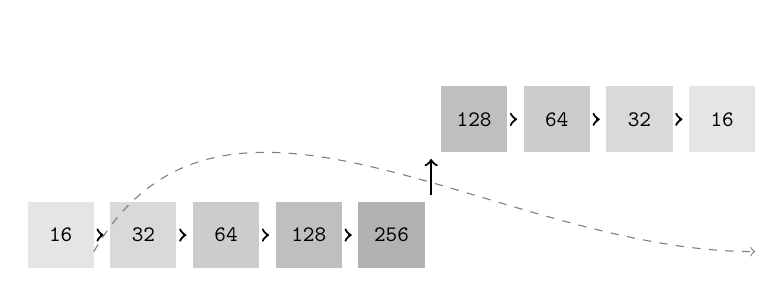
\begin{tikzpicture}[scale=0.42, every node/.style={scale=0.8,font=\ttfamily\bfseries}]
      \fill[gray!20] (0,0) rectangle (2,2);
      \fill[gray!30] (2.5,0) rectangle (4.5,2);
      \fill[gray!40] (5,0) rectangle (7,2);
      \fill[gray!50] (7.5,0) rectangle (9.5,2);
      \fill[gray!60] (10,0) rectangle (12,2);
      \fill[gray!50] (12.5,3.5) rectangle (14.5,5.5);
      \fill[gray!40] (15,3.5) rectangle (17,5.5);
      \fill[gray!30] (17.5,3.5) rectangle (19.5,5.5);
      \fill[gray!20] (20,3.5) rectangle (22,5.5);
      \draw (1,1) node {16};
      \draw (3.5,1) node {32};
      \draw (6,1) node {64};
      \draw (8.5,1) node {128};
      \draw (11,1) node {256};
      \draw (13.5,4.5) node {128};
      \draw (16,4.5) node {64};
      \draw (18.5,4.5) node {32};
      \draw (21,4.5) node {16};
      \draw[->,thick] (2.2,1) -- (2.3,1);
      \draw[->,thick] (4.7,1) -- (4.8,1);
      \draw[->,thick] (7.2,1) -- (7.3,1);
      \draw[->,thick] (9.7,1) -- (9.8,1);
      \draw[->,thick] (12.2,2.2) -- (12.2,3.3);
      \draw[->,thick] (14.7,4.5) -- (14.8,4.5);
      \draw[->,thick] (17.2,4.5) -- (17.3,4.5);
      \draw[->,thick] (19.7,4.5) -- (19.8,4.5);
      \draw[dashed,gray,->] (2,0.5) to[out=60,in=180] (22,0.5);
    \end{tikzpicture}
  \end{center}
  \vspace{0.3cm}
  \hfill\small (skip connections: encoder $\to$ decoder at same level)
  \vspace{0.2cm}
  \begin{columns}
    \column{0.5\textwidth}
      \begin{itemize}
        \item Channels: 16 $\to$ 32 $\to$ 64 $\to$ 128 $\to$ 256
        \item Block: DoubleConv (Conv3$\times$3, GroupNorm, ReLU)
      \end{itemize}
    \column{0.5\textwidth}
      \begin{itemize}
        \item Input: RGB + noise map (4 channels)
        \item Output: RGB + $\tanh$ (range $[-1,1]$)
        \item $\sim$1.9M parameters
      \end{itemize}
  \end{columns}
\end{frame}

\begin{frame}{UNet -- Training}
  \begin{columns}
    \column{0.48\textwidth}
      \begin{block}{Configuration}
        \begin{tabular}{ll}\toprule
          \textbf{Parameter} & \textbf{Value}\\\midrule
          Loss & L1 (MAE)\\
          Optimizer & Adam\\
          Learning rate & $10^{-4}$\\
          Batch size & 16\\
          Epochs & 50\\
          Noise aug. & Uniform $\sigma_n$\\\bottomrule
        \end{tabular}
      \end{block}
      \vspace{0.2cm}
      \textbf{Multi-noise augmentation:}
      random $\sigma_n$ per batch
      \begin{itemize}
        \item Robust model across all noise levels
        \item Avoids overfitting to a single $\sigma_n$
      \end{itemize}
    \column{0.52\textwidth}
      \small
      \textbf{Training pseudo-code:}
      \vspace{0.15cm}
      \begin{enumerate}
        \item \textbf{for} epoch $=1$ \textbf{to} $50$ \textbf{do}
        \item \hspace{0.5cm}\textbf{for} batch $b$ \textbf{in} train\_loader \textbf{do}
        \item \hspace{1.0cm}$\sigma \gets \text{Uniform}\{\sigma_n\}$
        \item \hspace{1.0cm}$\tilde{b} \gets \text{degrade}(b, \sigma)$
        \item \hspace{1.0cm}$\hat{b} \gets \text{UNet}(\tilde{b})$ \hfill\tiny forward
        \item \hspace{1.0cm}$\mathcal{L} \gets \|\hat{b} - b\|_1$ \hfill\tiny L1 loss
        \item \hspace{1.0cm}$\nabla_\theta\mathcal{L} \gets$ backprop \hfill\tiny backward
        \item \hspace{1.0cm}$\theta \gets$ AdamStep$(\theta)$ \hfill\tiny update
        \item \hspace{0.5cm}\textbf{end for}
        \item \hspace{0.5cm}val\_psnr $\gets$ validate(model)
        \item \hspace{0.5cm}save if val\_psnr $>$ best
        \item \textbf{end for}
      \end{enumerate}
      \vspace{0.2cm}
      \small
      \textbf{Checkpoint:} \texttt{results/unet/best\_model.pth}
  \end{columns}
\end{frame}

\begin{frame}{UNet -- Results}
  \begin{columns}
    \column{0.5\textwidth}
      \textbf{PSNR and SSIM on 145 test images}
      \vspace{0.2cm}
      \begin{tabular}{l|ccc}\toprule
        $\sigma_n$ & \textbf{PSNR} & \textbf{SSIM} & \textbf{Time}\\\midrule
         0.005 & 29.79 & 0.896 & 0.030 s\\
         0.01  & 29.79 & 0.895 & 0.028 s\\
         0.05  & 29.44 & 0.864 & 0.027 s\\
         0.1   & 28.46 & 0.795 & 0.026 s\\\bottomrule
      \end{tabular}
      \vspace{0.3cm}
      \begin{itemize}
        \item Minimal degradation ($\sim$1 dB between extremes)
        \item \textbf{Surpasses TV} at $\sigma_n=0.1$ (28.46 vs 26.54 dB)
        \item Fastest inference: 0.030 s/img
      \end{itemize}
    \column{0.5\textwidth}
      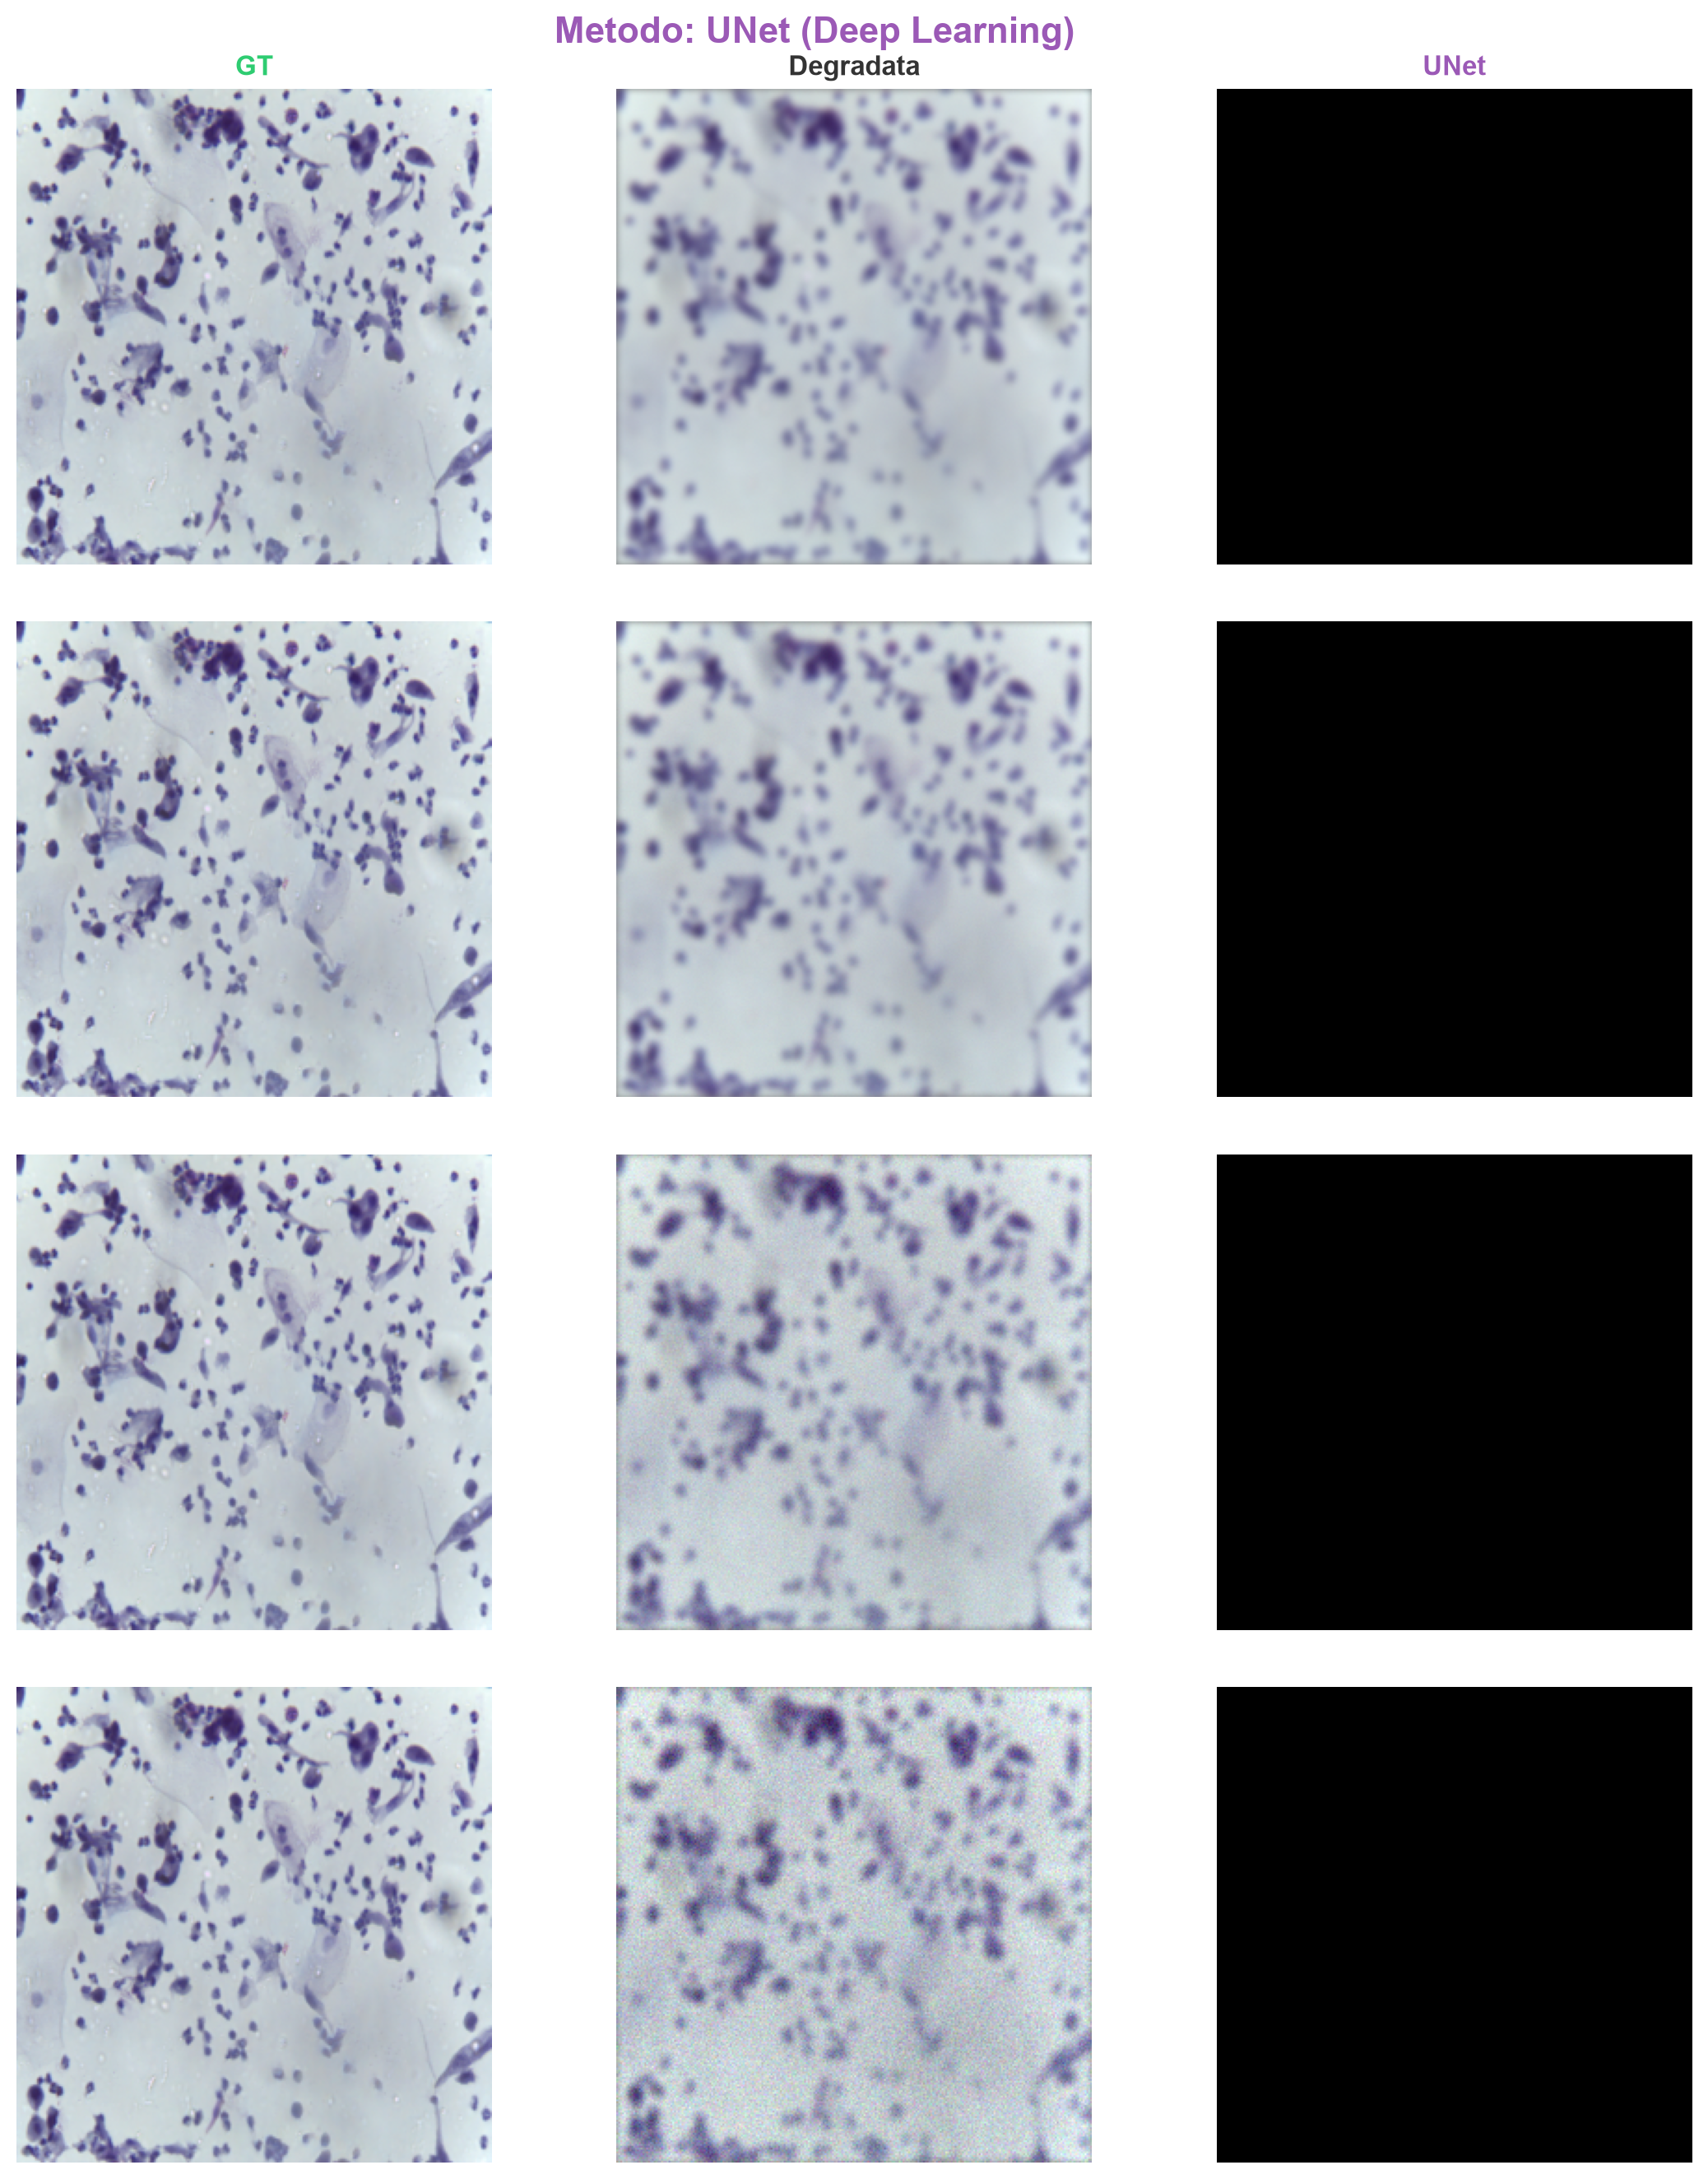
\includegraphics[width=\textwidth]{../results/qualitative_slides/unet_comparison.png}
  \end{columns}
\end{frame}

\section{DiffPIR}

\begin{frame}{DiffPIR -- Overview}
  \begin{block}{DiffPIR (Diffusion-based Plug-and-Play Image Restoration)}
    \begin{itemize}
      \item Integrates a \textbf{diffusion model} (DDPM) into a Plug-and-Play framework
      \item Alternates \textbf{denoising} (generative prior) and \textbf{data-fidelity} (via FFT)
    \end{itemize}
  \end{block}
  \begin{alertblock}{Custom LightUNet (1.26M params, $\sim$5 MB)}
    Trained from scratch on 673 cervical LBC images\\[0.1cm]
    $\triangleright$ Specific to the cytological domain \\[0.1cm]
    $\triangleright$ Training on GPU (Apple MPS), inference $\sim$0.64\,s/img
  \end{alertblock}
\end{frame}

\begin{frame}{DDPM and LightUNet}
  \begin{columns}
    \column{0.55\textwidth}
      \textbf{Denoising Diffusion Probabilistic Models}
      \begin{itemize}\small
        \item 1000 timesteps, $\beta_1=10^{-4}$, $\beta_T=0.02$
        \item Loss: MSE on $\varepsilon_\theta(x_t,t)$
        \item Training: 673 images, 50 epochs
      \end{itemize}
      \vspace{0.2cm}
      \textbf{LightUNet}
      \begin{itemize}\small
        \item Base channels: 32
        \item Encoder: 32$\to$64$\to$128
        \item Sinusoidal time embedding + MLP
        \item GroupNorm + SiLU
        \item \textbf{1,262,273 parameters}
      \end{itemize}
    \column{0.45\textwidth}
      \begin{block}{Diffusion Process}
        \centering\small
        $x_0 \to x_1 \to \cdots \to x_T$ \\[0.1cm]
        \textbf{Forward} \\
        $q(x_t|x_{t-1}) = \mathcal{N}(\sqrt{1-\beta_t}x_{t-1}, \beta_t I)$ \\[0.2cm]
        \textbf{Reverse} \\
        $p_\theta(x_{t-1}|x_t) = \mathcal{N}(\mu_\theta(x_t,t), \Sigma_\theta(x_t,t))$
      \end{block}
  \end{columns}
\end{frame}

\begin{frame}{DiffPIR Algorithm}
  \begin{columns}
    \column{0.55\textwidth}
      \small
      \textbf{Pseudo-code:}
      \vspace{0.1cm}
      \begin{enumerate}
        \item $y \gets$ degraded image
        \item $\mathcal{K} \gets \text{FFT}(k)$ \hfill\tiny kernel OTF
        \item \textbf{for} $t = t_{\text{start}}$ \textbf{to} $1$ \textbf{do}
        \item \hspace{0.5cm}$\varepsilon \gets \varepsilon_\theta(x_t, t)$ \hfill\tiny DDPM denoise
        \item \hspace{0.5cm}$\hat{x}_0 \gets \frac{x_t - \sqrt{1-\bar{\alpha}_t}\,\varepsilon}{\sqrt{\bar{\alpha}_t}}$
        \item \hspace{0.5cm}$\hat{x}_0 \gets \text{clamp}(\hat{x}_0, -1, 1)$
        \item \hspace{0.5cm}$\rho_t \gets \lambda \cdot \frac{\sigma^2 \bar{\alpha}_t}{1 - \bar{\alpha}_t}$
        \item \hspace{0.5cm}$\tilde{x}_0 \gets \mathcal{F}^{-1}\!\left(\frac{\mathcal{F}(y)\overline{\mathcal{K}} + \rho_t\mathcal{F}(\hat{x}_0)}{|\mathcal{K}|^2 + \rho_t}\right)$
        \item \hspace{0.5cm}$x_{t-1} \gets$ DDIM step$(x_t, \tilde{x}_0)$
        \item \textbf{end for}
        \item \textbf{return} $x_0$
      \end{enumerate}
    \column{0.45\textwidth}
      \small
      \textbf{Step 1 -- Denoising:}
      \begin{equation*}
        \hat{x}_0^{(t)} = \frac{x_t - \sqrt{1-\bar{\alpha}_t}\,\varepsilon_\theta(x_t,t)}{\sqrt{\bar{\alpha}_t}}
      \end{equation*}
      \vspace{0.15cm}
      \textbf{Step 2 -- Data Fidelity (FFT):}
      \begin{equation*}
        \tilde{x}_0 = \mathcal{F}^{-1}\!\left(
        \frac{\mathcal{F}(y)\overline{\mathcal{F}(k)} + \rho\mathcal{F}(\hat{x}_0)}
             {|\mathcal{F}(k)|^2 + \rho}\right)
      \end{equation*}
      \vspace{0.15cm}
      \textbf{Dynamic weight:}
      \begin{equation*}
        \rho_t = \lambda \cdot \frac{\sigma^2 \cdot \bar{\alpha}_t}{1 - \bar{\alpha}_t}
      \end{equation*}
  \end{columns}
\end{frame}

\begin{frame}{DiffPIR -- Parameters and Results}
  \begin{columns}[T]
    \column{0.45\textwidth}
      \textbf{Heuristic parameter selection}\\[0.15cm]
      \centering
      \begin{tabular}{lc}\toprule
        \textbf{Parameter} & \textbf{Value}\\\midrule
        $t_{\text{start}}$       & 50 \\
        $\lambda$                & 10.0 \\
        \texttt{num\_steps}      & 15 \\
        $\zeta$                  & 0.0 (DDIM) \\\bottomrule
      \end{tabular}

      \vspace{0.4cm}
      \raggedright\textbf{Quantitative results}\\[0.15cm]
      \centering
      \begin{tabular}{c|cc}\toprule
        $\sigma_n$ & \textbf{PSNR} & \textbf{SSIM}\\\midrule
        0.005 & 15.80 & 0.356\\
        0.01  & 16.48 & 0.407\\
        0.05  & 22.77 & 0.722\\
        0.1   & 25.60 & 0.797\\\bottomrule
      \end{tabular}

      \vspace{0.25cm}
      \raggedright
      \begin{itemize}\small
        \item PSNR \textbf{increases} with noise
        \item Best at $\sigma_n=0.1$ (25.60 dB)
      \end{itemize}

    \column{0.55\textwidth}
      \centering
      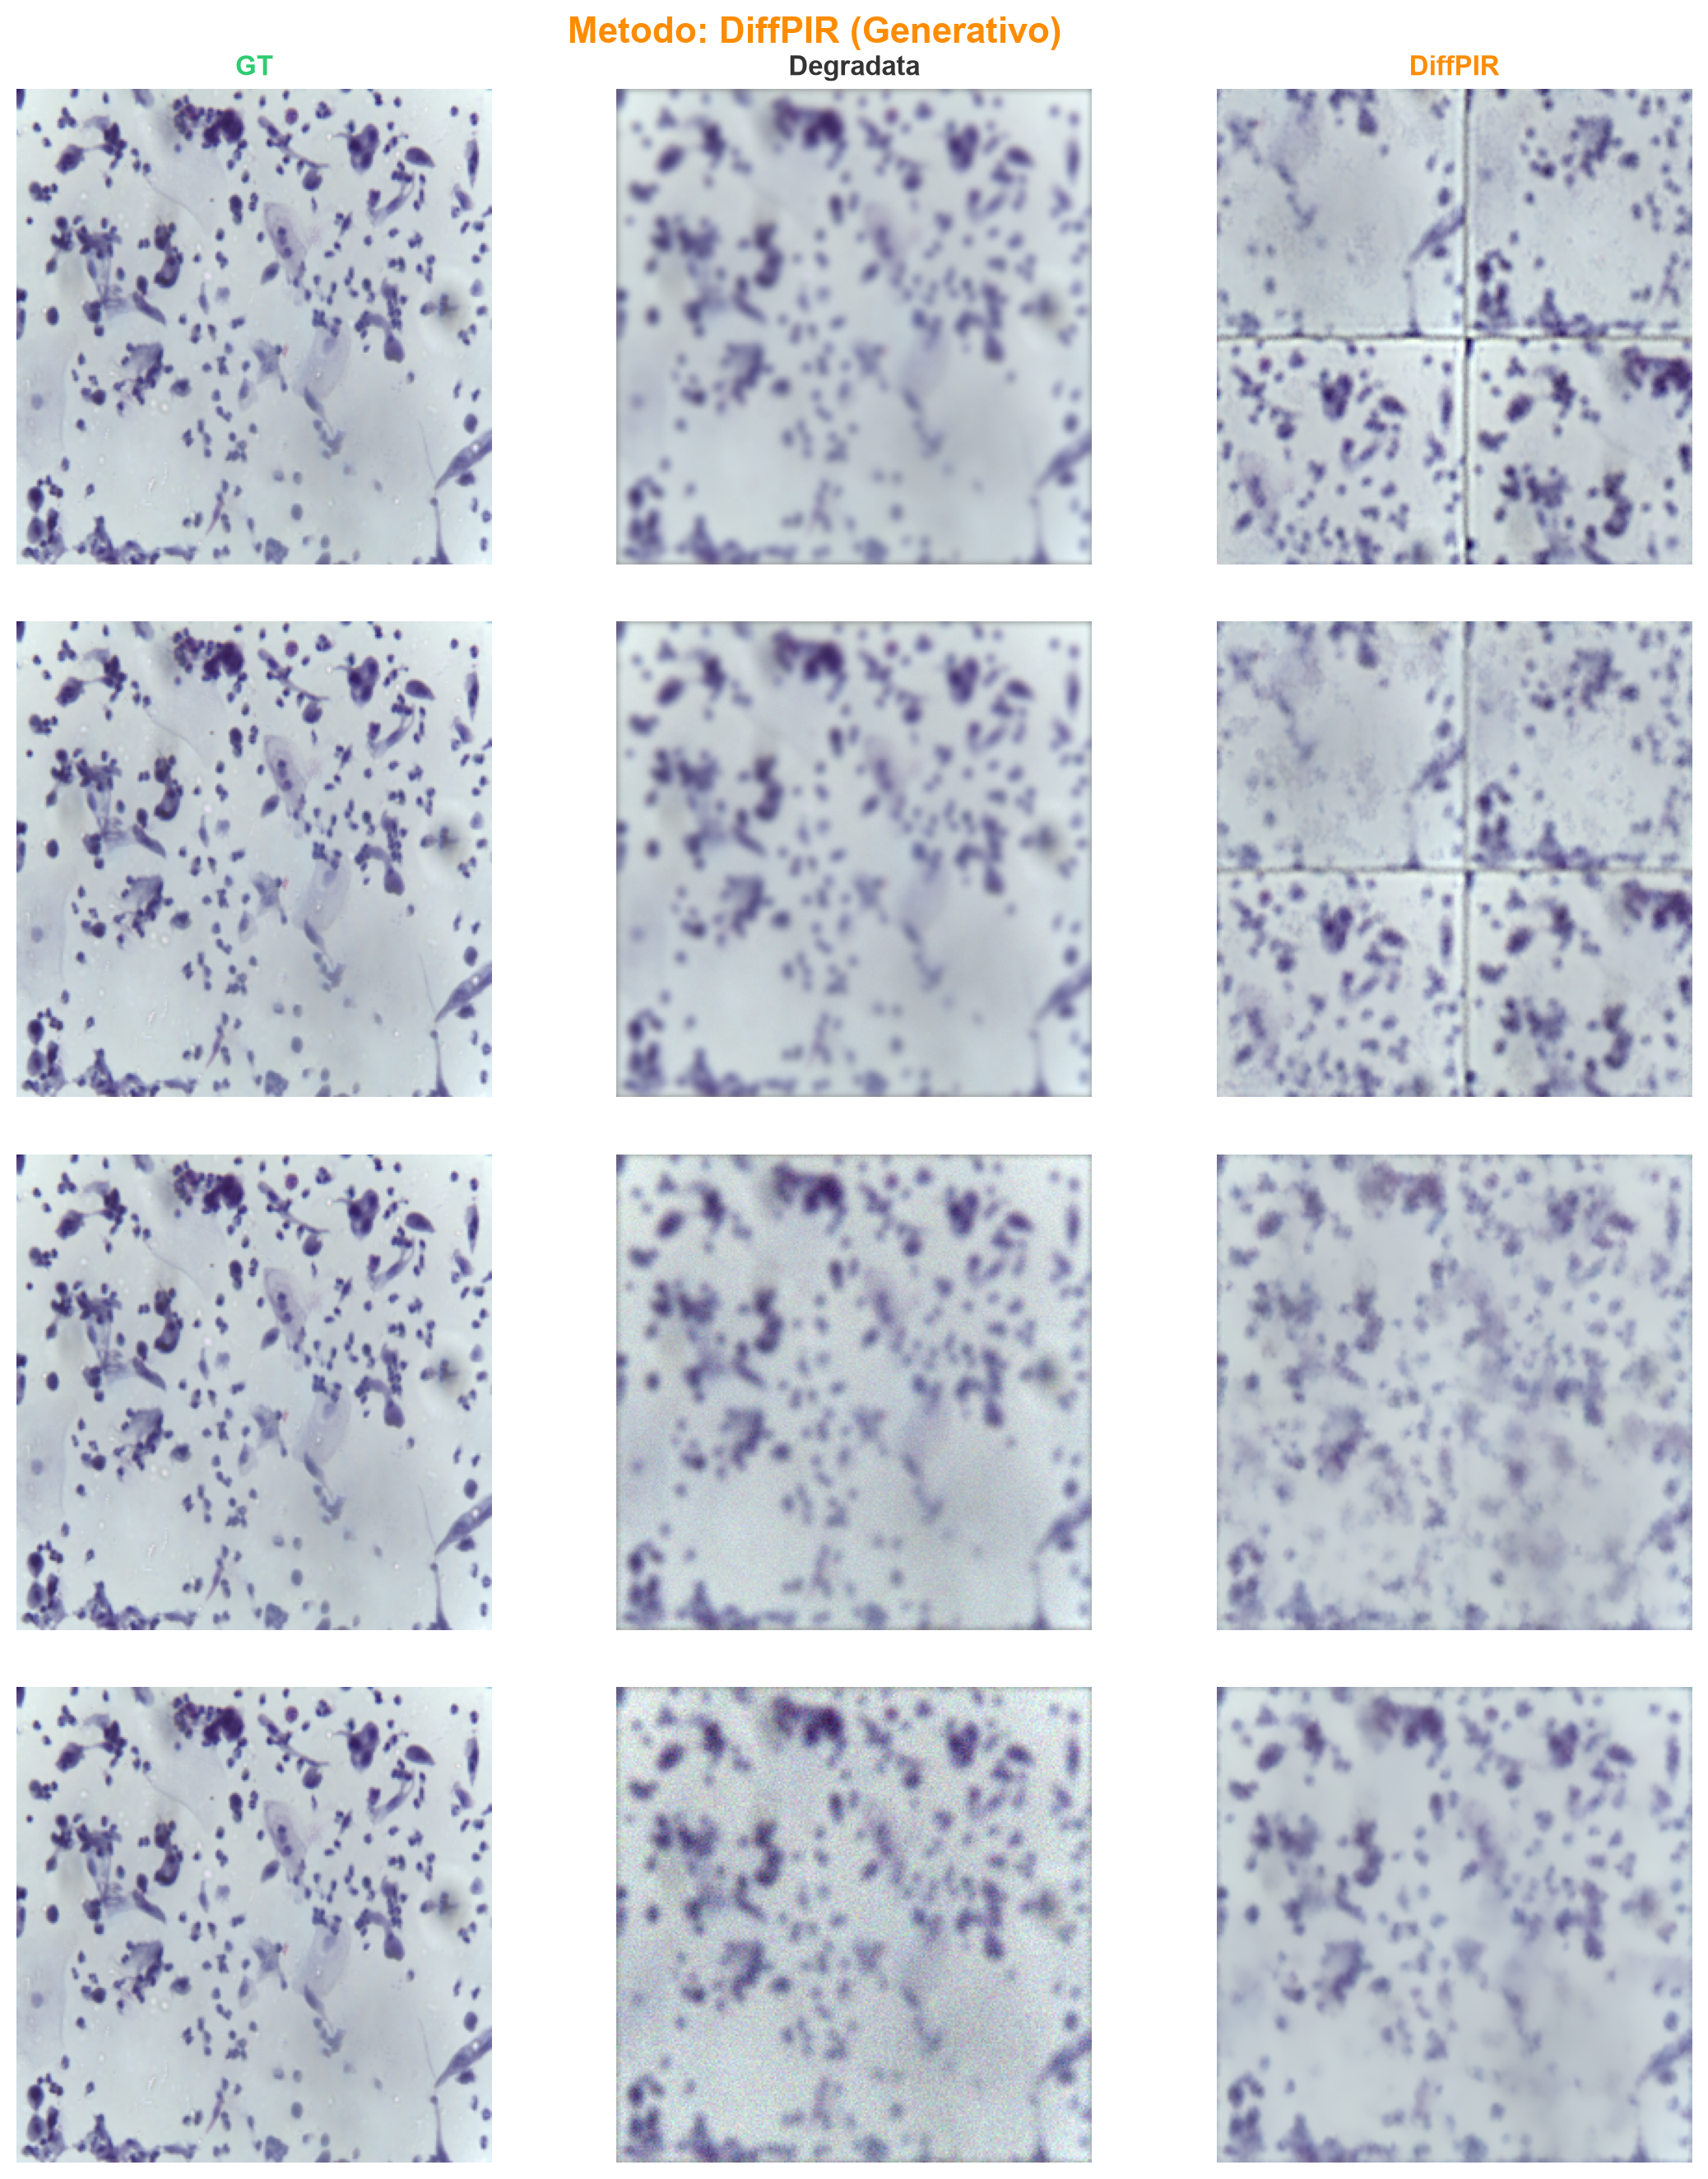
\includegraphics[width=\textwidth]{../results/qualitative_slides/diffpir_comparison.png}
  \end{columns}
\end{frame}


\section{Quantitative Results}

\begin{frame}{PSNR / SSIM Comparison}
  \small
  \begin{tabular}{l|ccc|ccc}\toprule
    & \multicolumn{3}{c|}{\textbf{PSNR (dB) $\uparrow$}} & \multicolumn{3}{c}{\textbf{SSIM $\uparrow$}}\\
    $\sigma_n$ & \textbf{TV} & \textbf{UNet} & \textbf{DiffPIR} & \textbf{TV} & \textbf{UNet} & \textbf{DiffPIR}\\\midrule
     0.005 & \textbf{32.09} & 29.79 & 15.80 & \textbf{0.911} & 0.896 & 0.356\\
     0.01  & \textbf{32.04} & 29.79 & 16.48 & \textbf{0.909} & 0.895 & 0.407\\
     0.05  & \textbf{30.42} & 29.44 & 22.77 & 0.837 & \textbf{0.864} & 0.722\\
     0.1   & 26.54 & \textbf{28.46} & 25.60 & 0.586 & \textbf{0.795} & 0.797\\\bottomrule
  \end{tabular}
  \vspace{0.3cm}
  \begin{block}{Observations}
    \begin{itemize}
      \item \textbf{TV}: dominates at $\sigma_n\leq0.01$ (PSNR $>$ 32 dB, SSIM $>$ 0.9)
      \item \textbf{UNet}: best trade-off, $\sim$1 dB degradation, surpasses TV at $\sigma_n=0.1$
      \item \textbf{DiffPIR}: generative, PSNR increases with noise (15.80$\to$25.60 dB)
    \end{itemize}
  \end{block}
\end{frame}

\begin{frame}{Comparative Graph}
  \begin{center}
    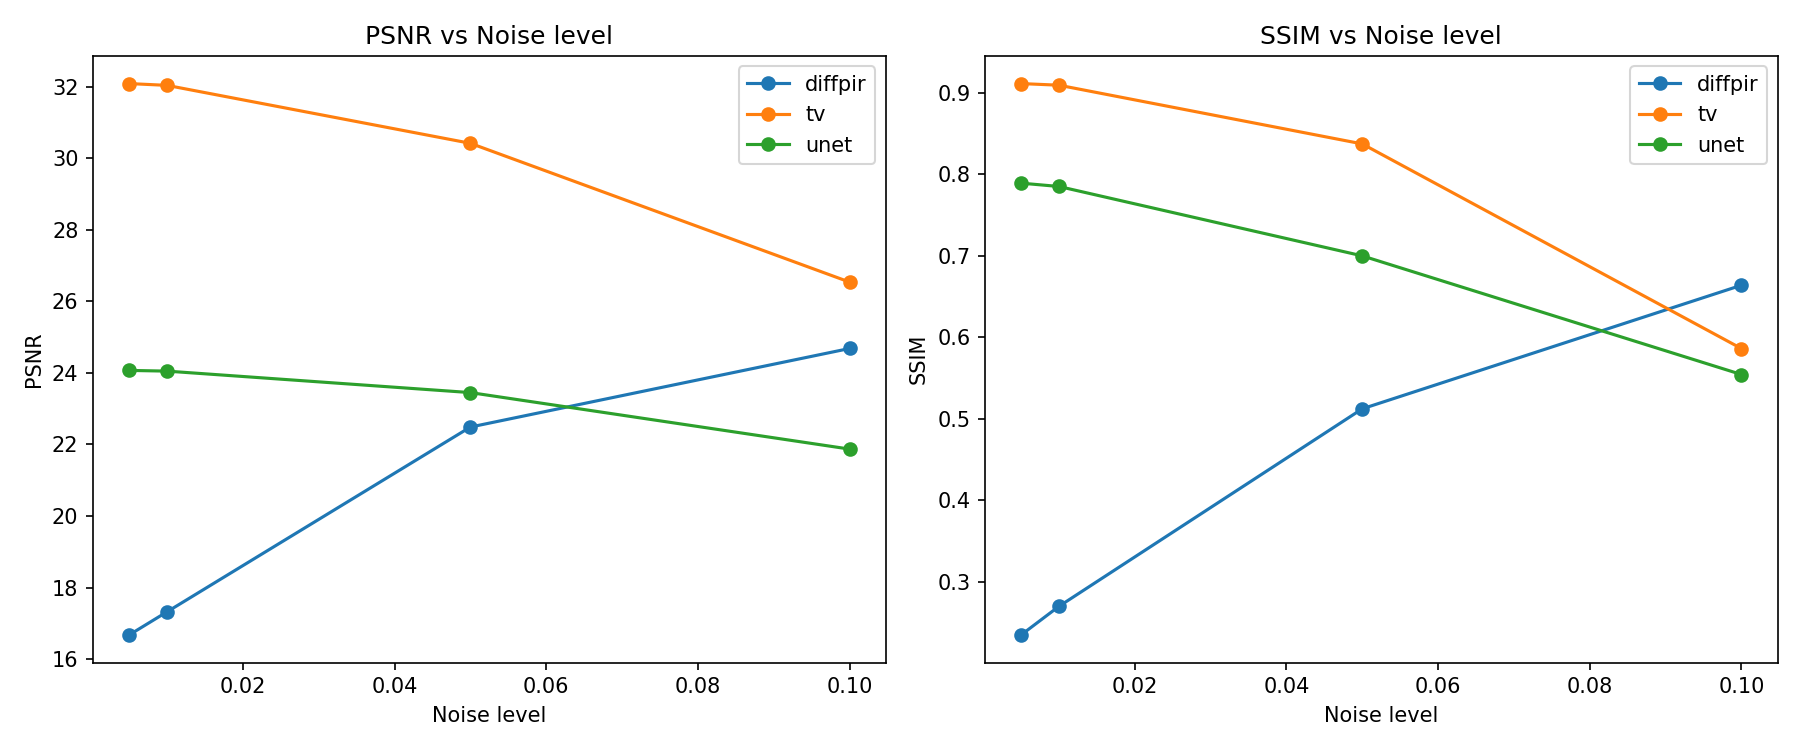
\includegraphics[width=0.92\textwidth]{../results/comparison.png}
  \end{center}
\end{frame}

\section{Qualitative Results}

\begin{frame}{Full Grid}
  \begin{center}
    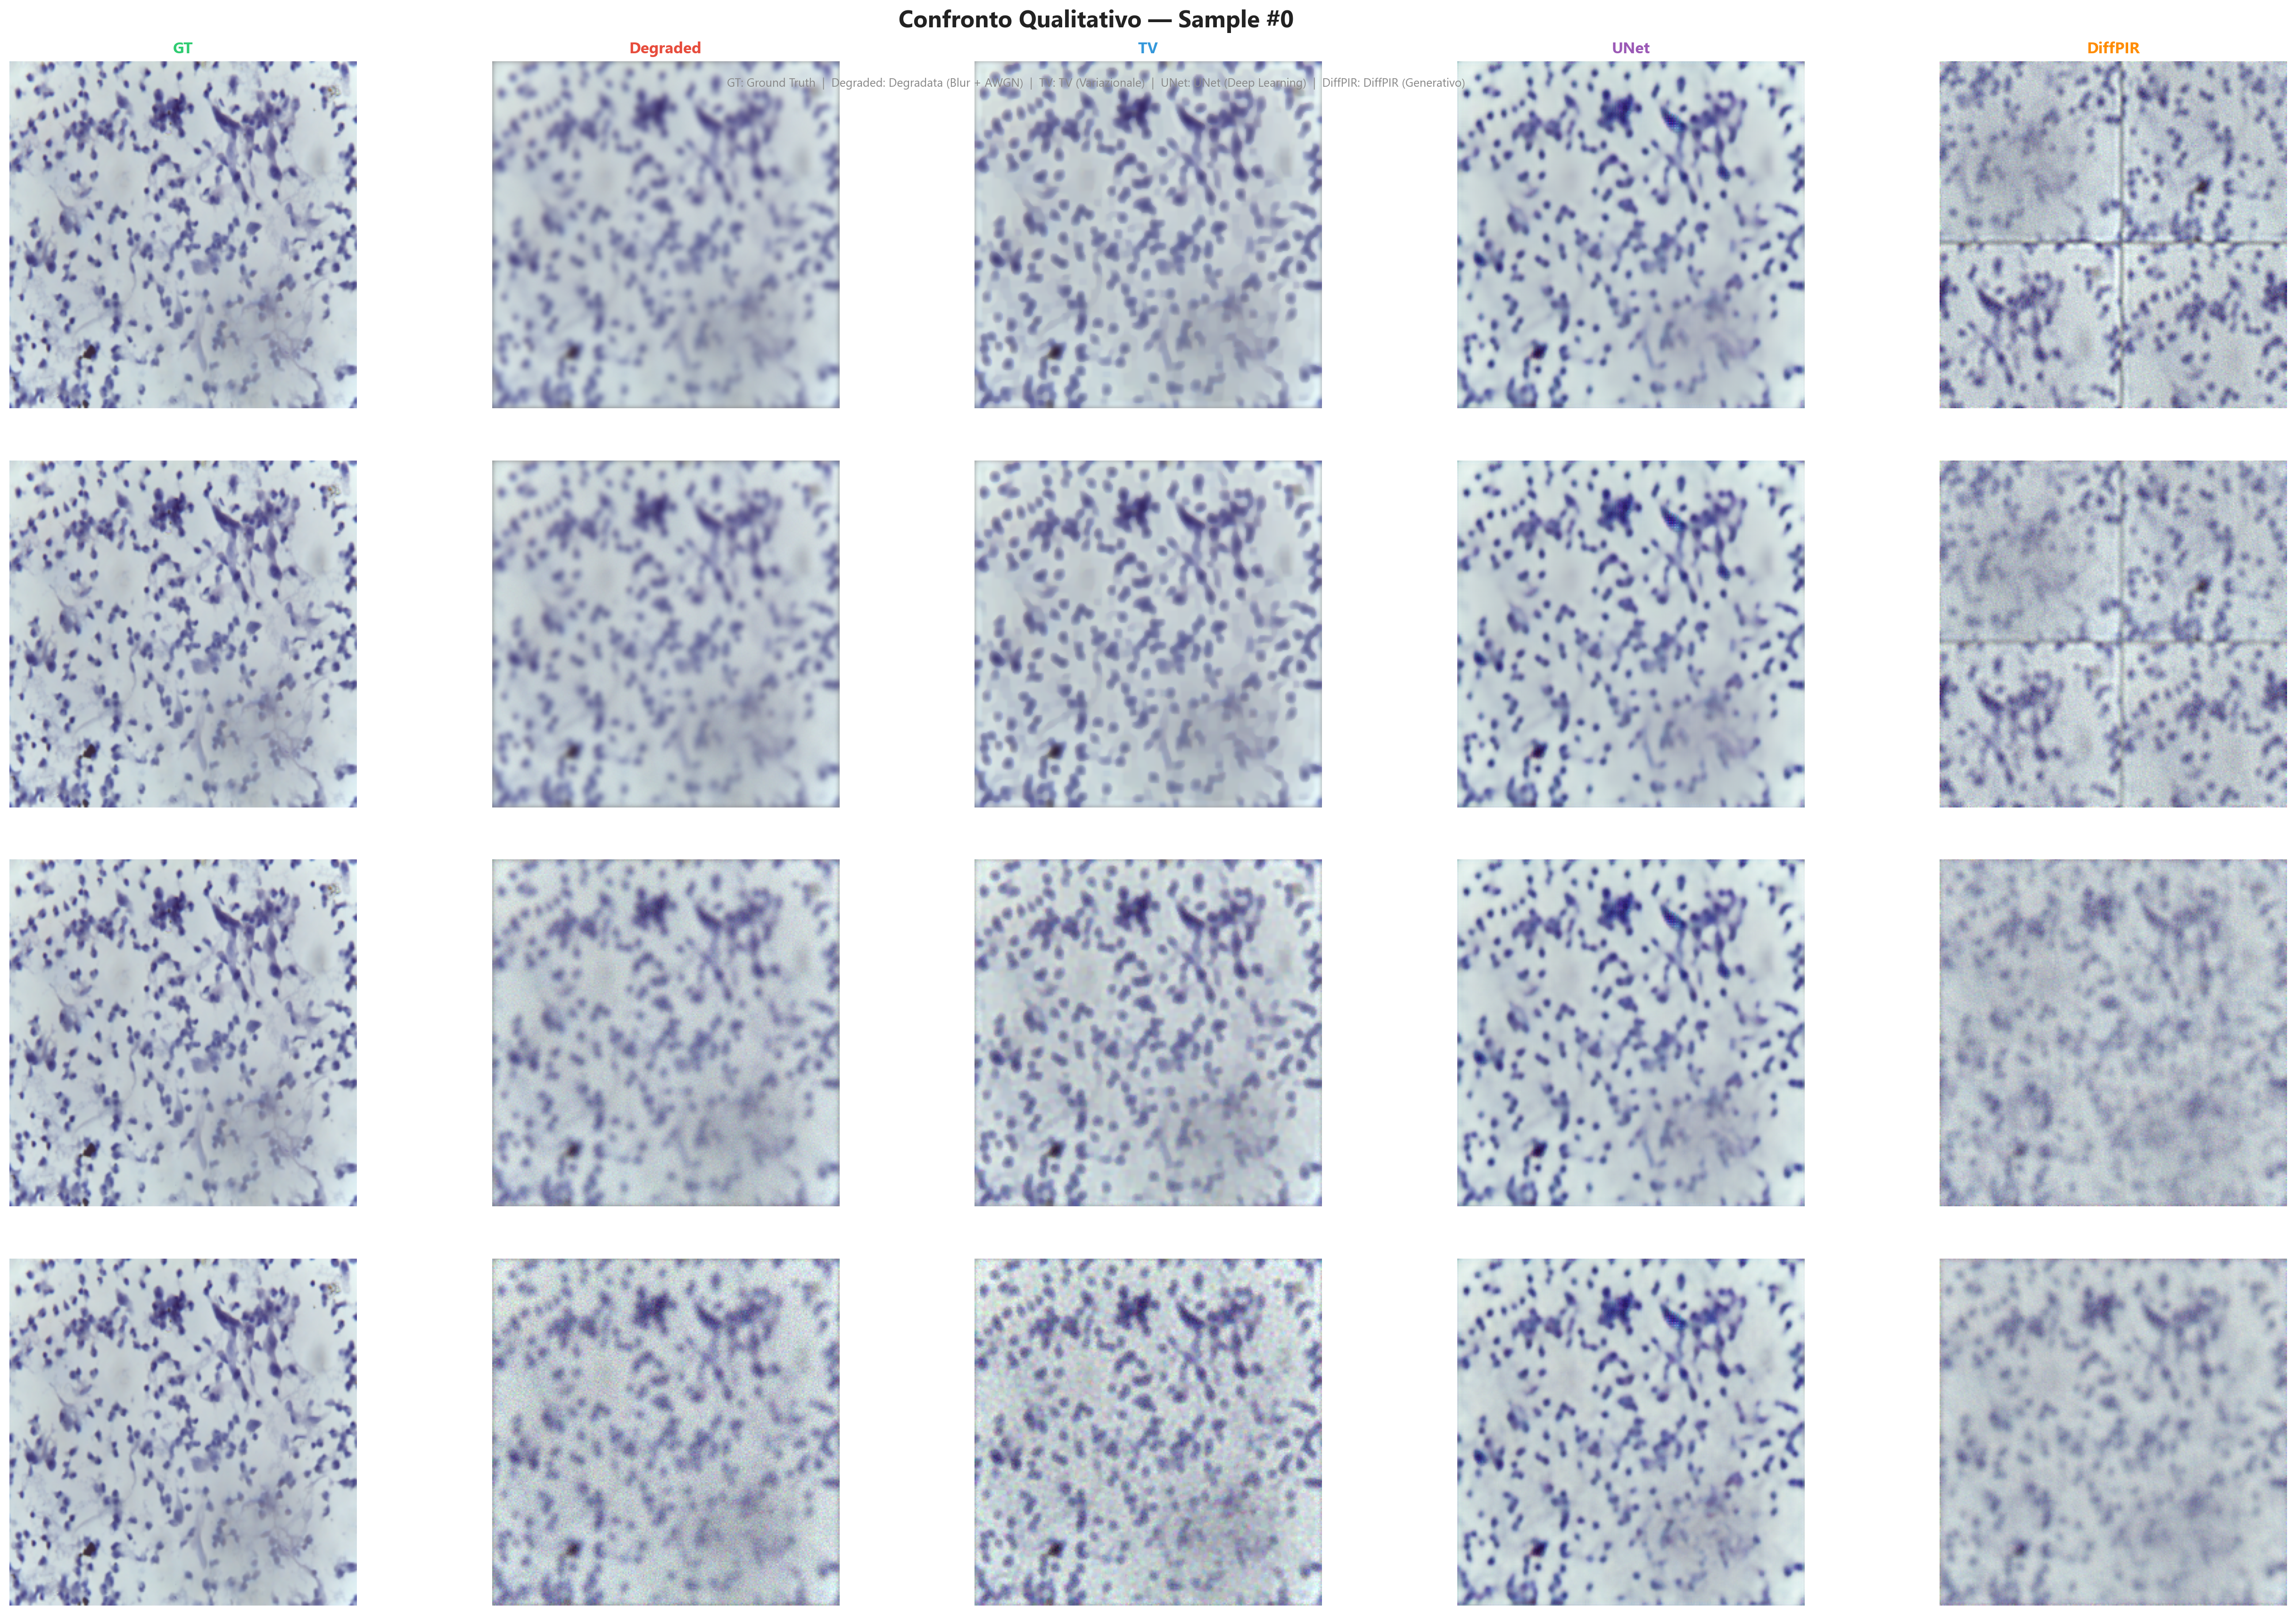
\includegraphics[width=0.7\textwidth]{../results/qualitative_slides/all_methods_grid.png}
  \end{center}
\end{frame}

\begin{frame}{Visual Comparison -- $\sigma_n = 0.005$}
  \begin{center}
    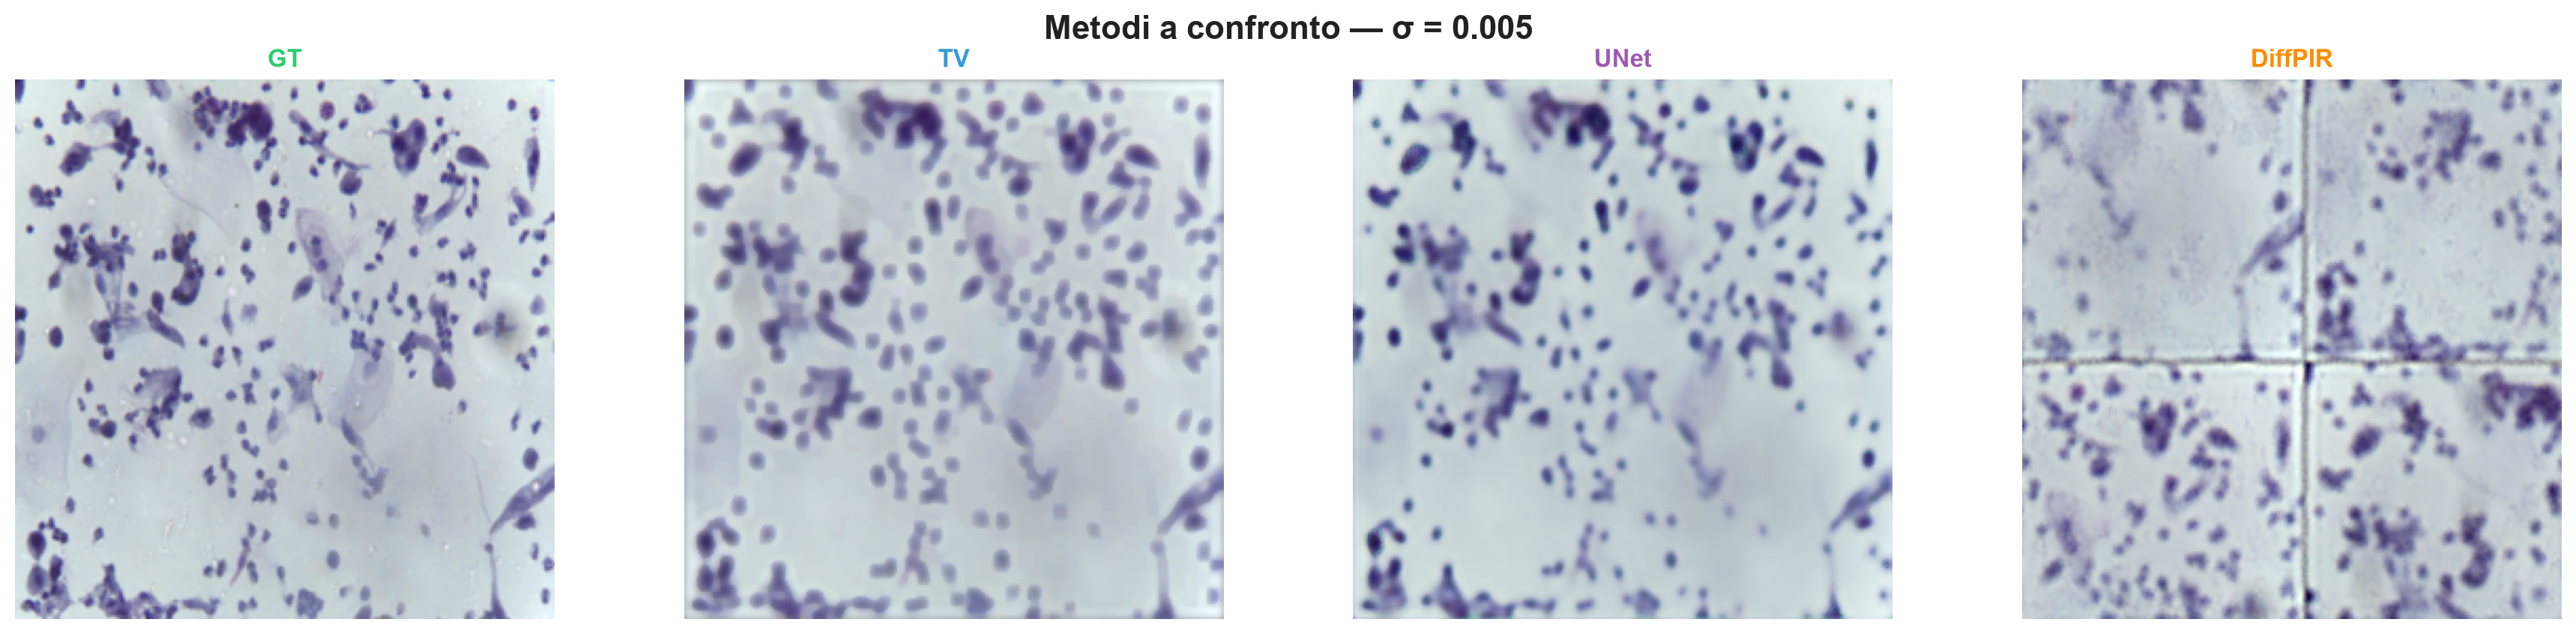
\includegraphics[width=0.95\textwidth]{../results/qualitative_slides/methods_noise_0.005.png}
    \vspace{0.2cm}
    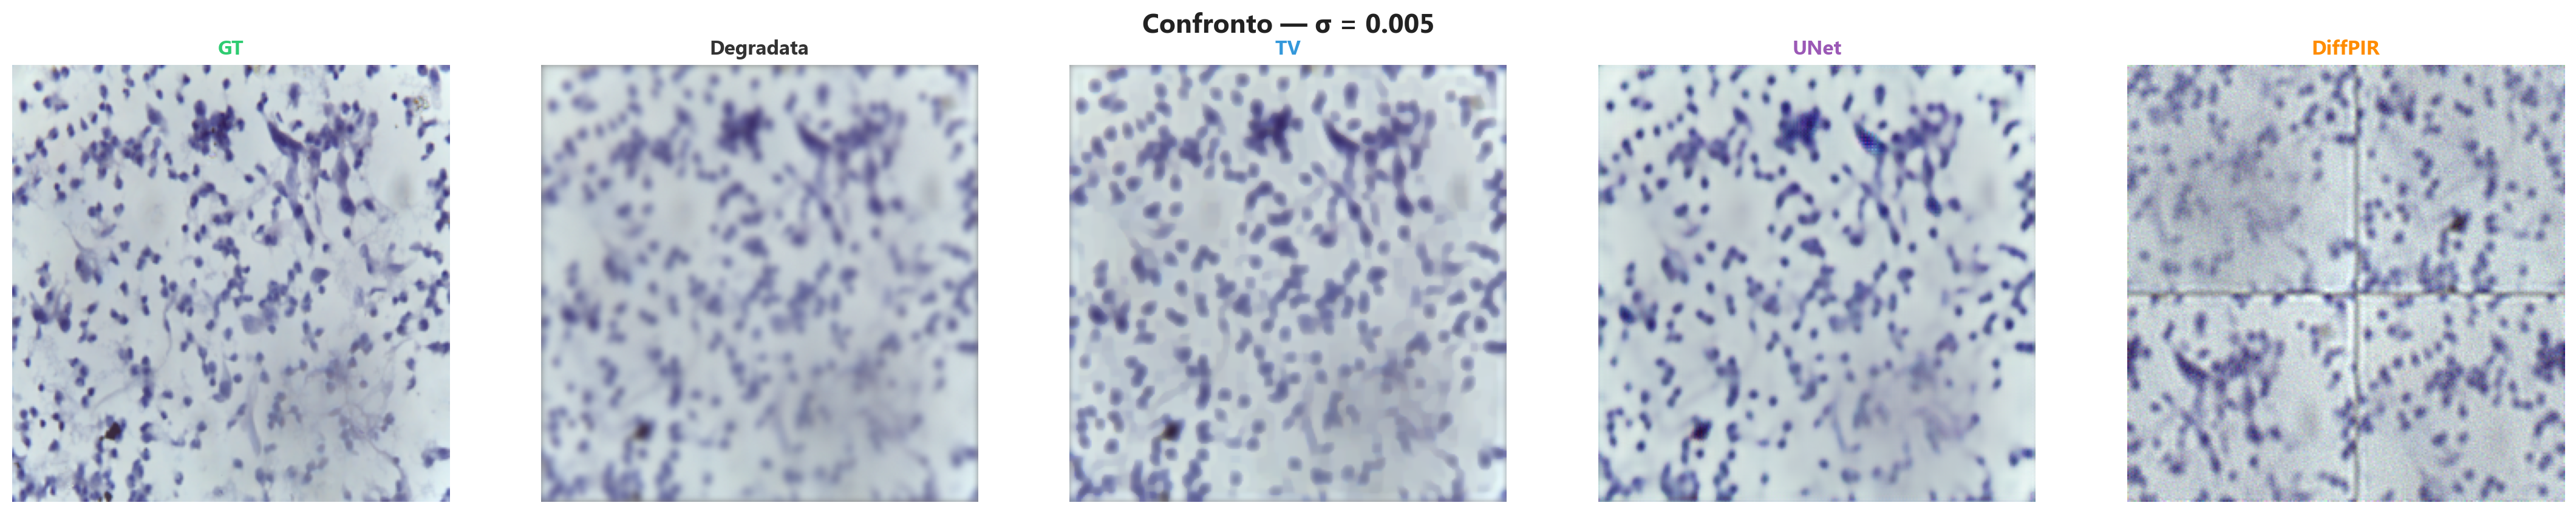
\includegraphics[width=0.95\textwidth]{../results/qualitative_slides/noise_0.005_comparison.png}
  \end{center}
\end{frame}

\begin{frame}{Visual Comparison -- $\sigma_n = 0.01$}
  \begin{center}
    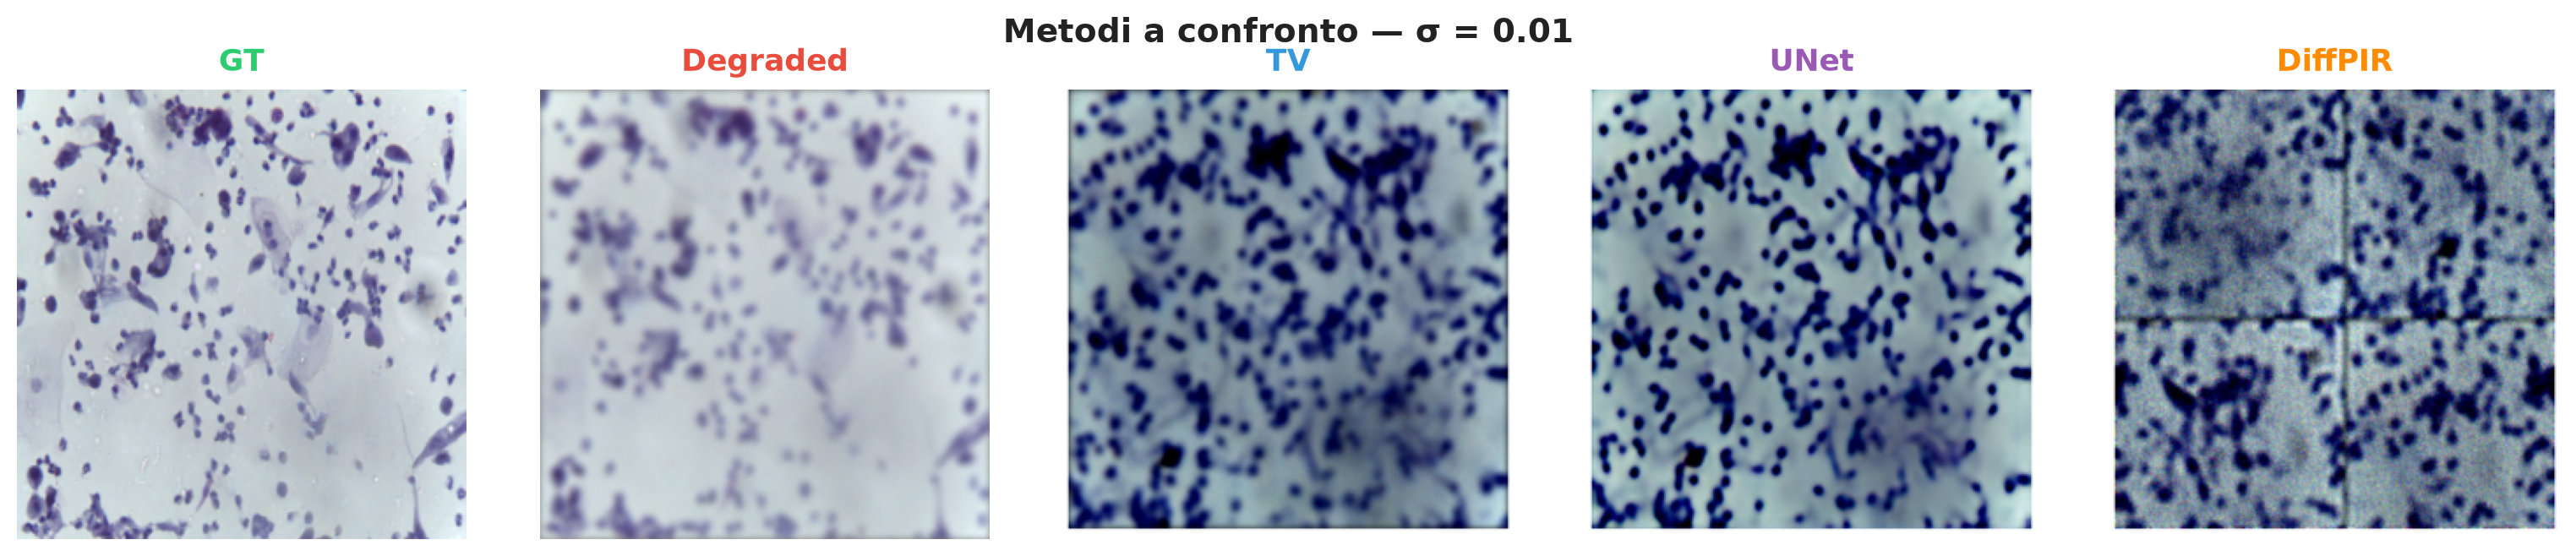
\includegraphics[width=0.95\textwidth]{../results/qualitative_slides/methods_noise_0.01.png}
    \vspace{0.2cm}
    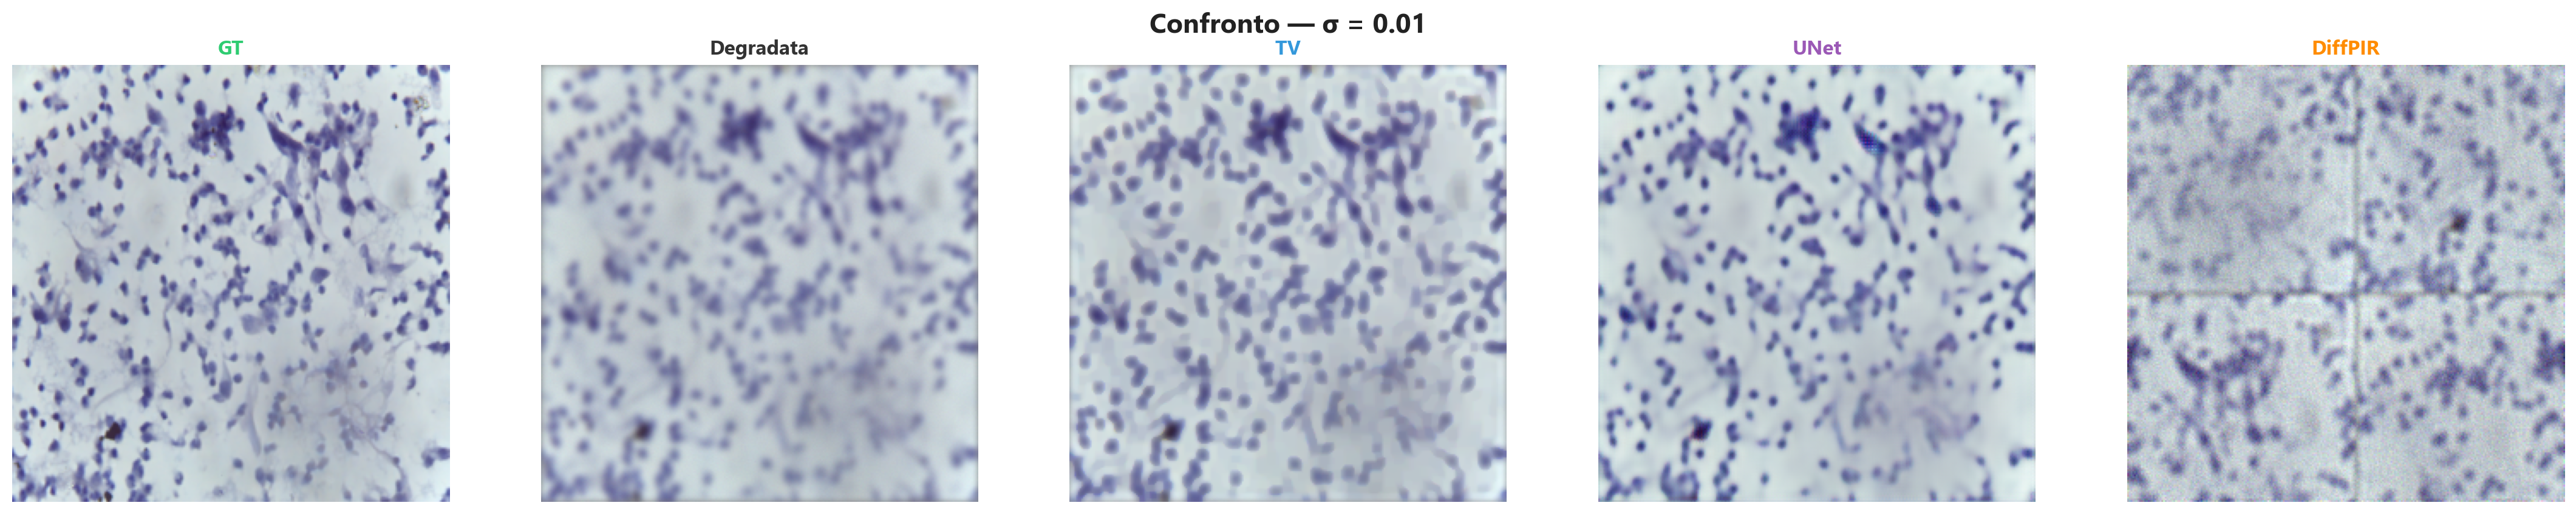
\includegraphics[width=0.95\textwidth]{../results/qualitative_slides/noise_0.01_comparison.png}
  \end{center}
\end{frame}

\begin{frame}{Visual Comparison -- $\sigma_n = 0.05$}
  \begin{center}
    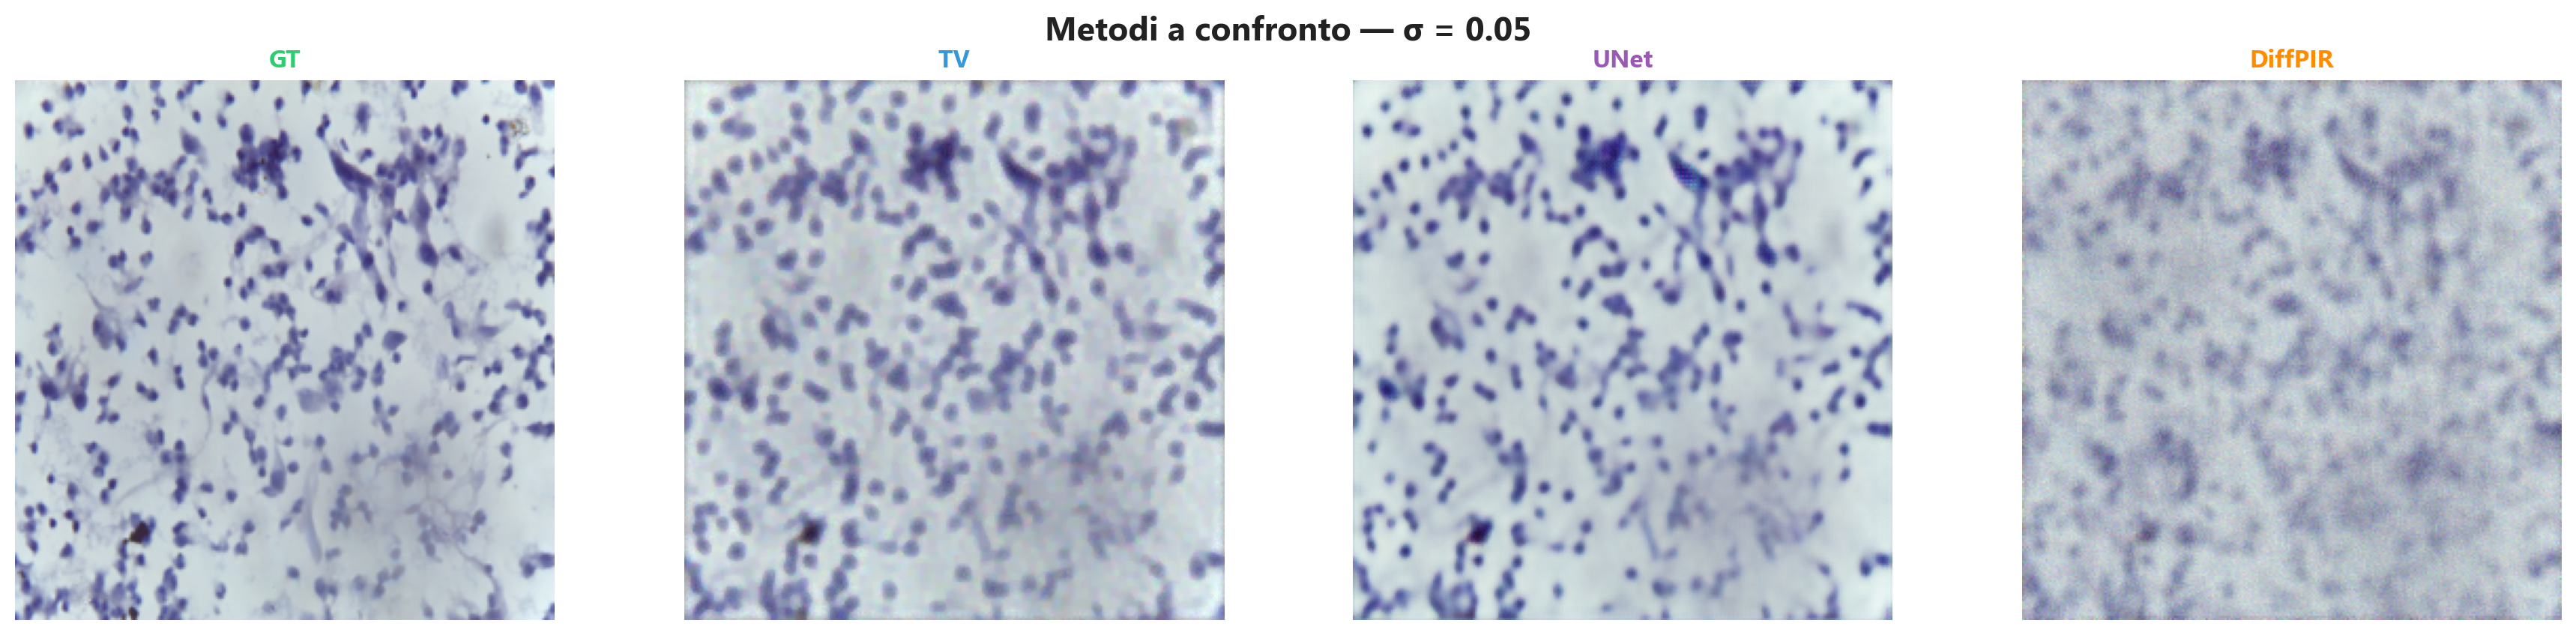
\includegraphics[width=0.95\textwidth]{../results/qualitative_slides/methods_noise_0.05.png}
    \vspace{0.3cm}
    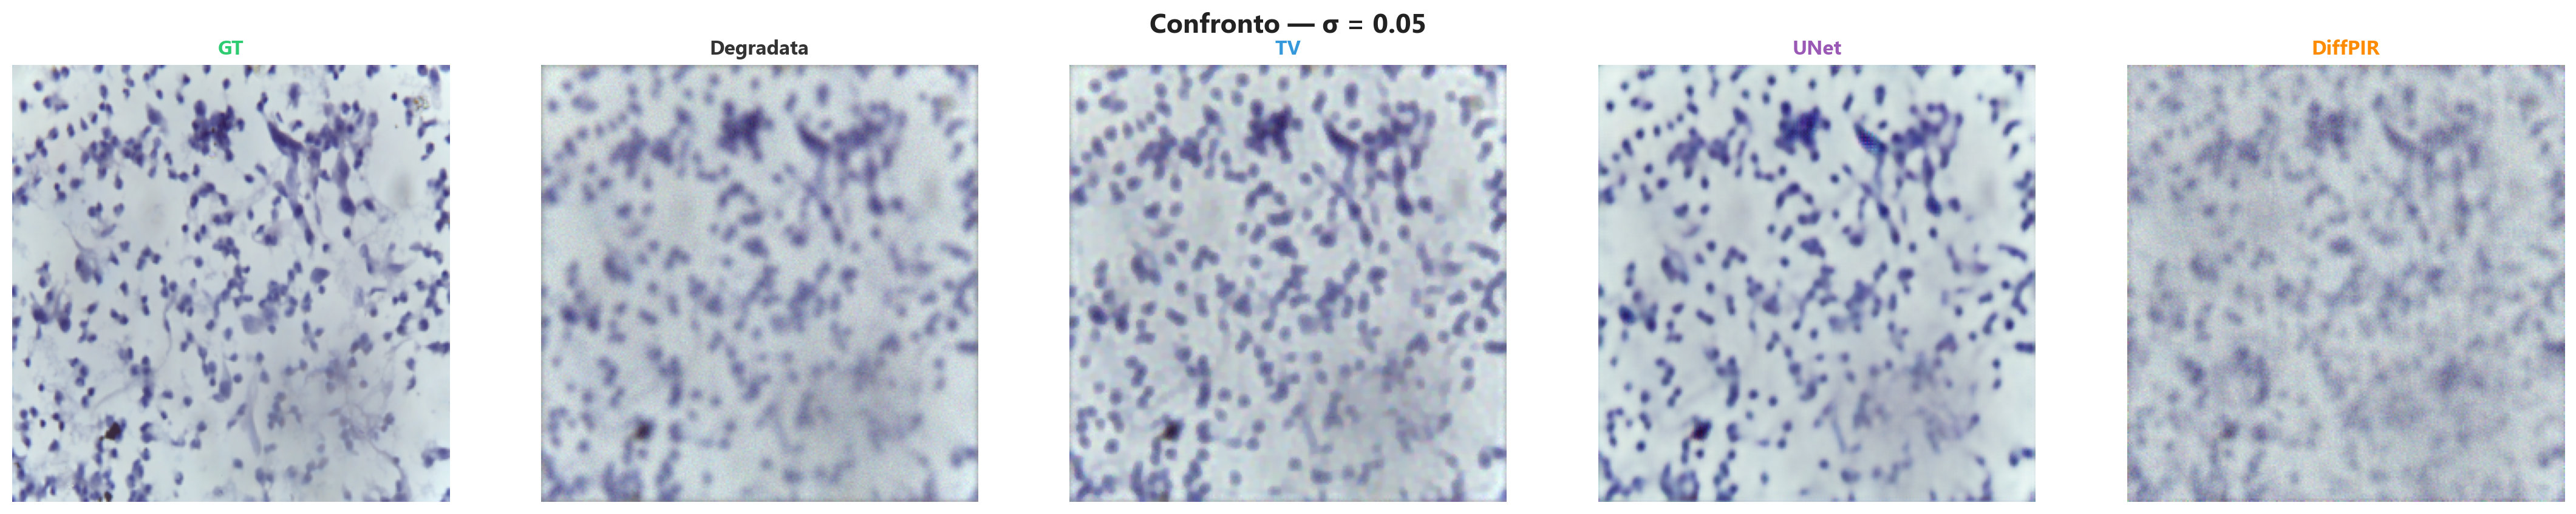
\includegraphics[width=0.74\textwidth]{../results/qualitative_slides/noise_0.05_comparison.png}
  \end{center}
\end{frame}

\begin{frame}{Visual Comparison -- $\sigma_n = 0.1$}
  \begin{center}
    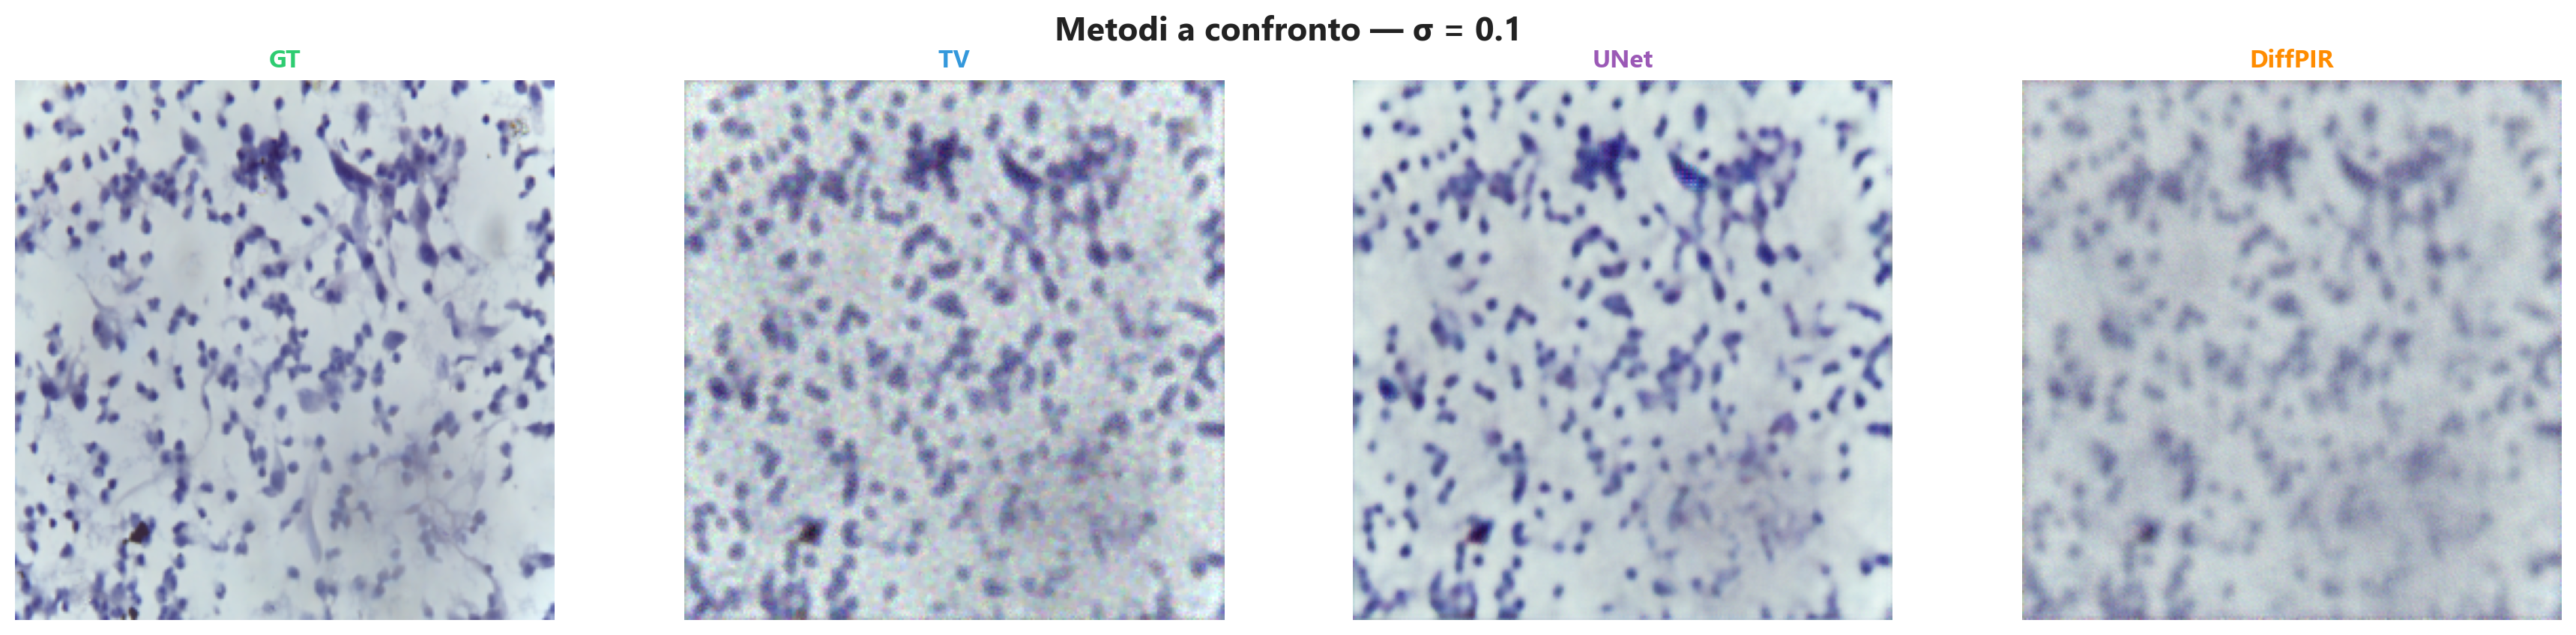
\includegraphics[width=0.95\textwidth]{../results/qualitative_slides/methods_noise_0.1.png}
    \vspace{0.2cm}
    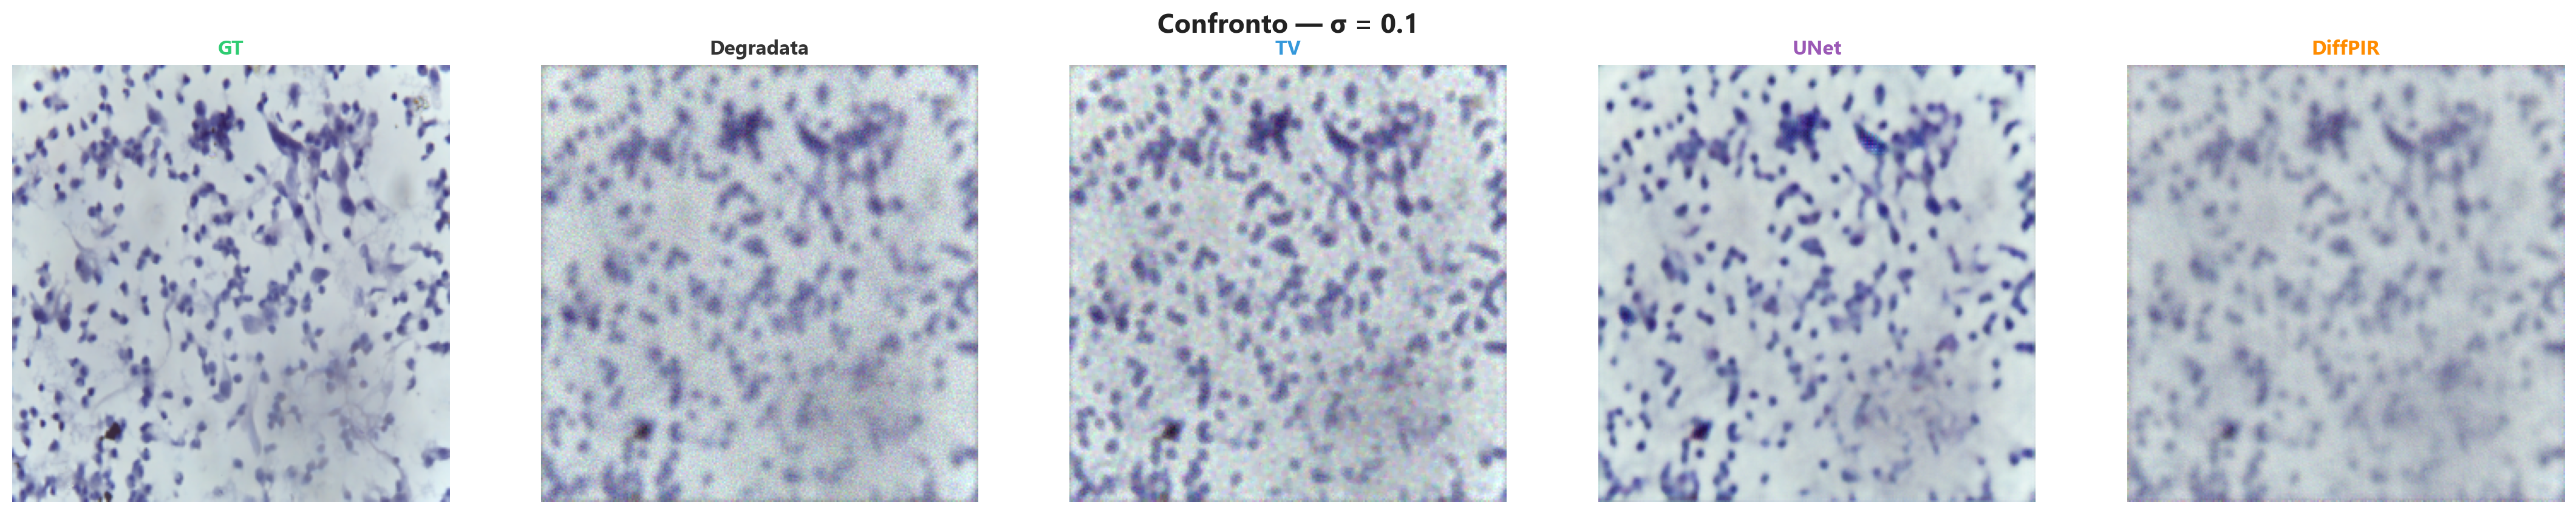
\includegraphics[width=0.95\textwidth]{../results/qualitative_slides/noise_0.1_comparison.png}
  \end{center}
\end{frame}

\section{Discussion}

\begin{frame}{Family Comparison}
  \begin{columns}[t]
    \column{0.48\textwidth}
      {\setbeamercolor{block title}{bg=darkblue,fg=white}%
       \setbeamercolor{block body}{bg=darkblue!5}%
      \begin{block}{\small\bfseries TV  \hfill \scriptsize\itshape Variational}
        \scriptsize
        \textcolor{green!50!black}{$\blacktriangleright$} \textbf{Pros}\\[0.05cm]
        \hspace{0.3cm}$\checkmark$ No training data required\\
        \hspace{0.3cm}$\checkmark$ Interpretable, unique solution\\
        \hspace{0.3cm}$\checkmark$ Robust at low noise ($\sigma_n \leq 0.01$)\\[0.08cm]
        \textcolor{red}{$\blacktriangleright$} \textbf{Cons}\\[0.05cm]
        \hspace{0.3cm}$\times$ Staircasing at high $\lambda$\\
        \hspace{0.3cm}$\times$ Degrades rapidly at high $\sigma_n$
      \end{block}}

    \column{0.48\textwidth}
      {\setbeamercolor{block title}{bg=green!45!black,fg=white}%
       \setbeamercolor{block body}{bg=green!5}%
      \begin{block}{\small\bfseries UNet  \hfill \scriptsize\itshape Deep Learning}
        \scriptsize
        \textcolor{green!50!black}{$\blacktriangleright$} \textbf{Pros}\\[0.05cm]
        \hspace{0.3cm}$\checkmark$ Very fast inference (0.030\,s/img)\\
        \hspace{0.3cm}$\checkmark$ Robust across the spectrum ($\Delta$PSNR $\sim$1\,dB)\\[0.08cm]
        \textcolor{red}{$\blacktriangleright$} \textbf{Cons}\\[0.05cm]
        \hspace{0.3cm}$\times$ Requires supervised training\\
        \hspace{0.3cm}$\times$ Limited generalization outside domain
      \end{block}}
  \end{columns}

  \vspace{0.25cm}

  \begin{columns}[t]
    \column{0.70\textwidth}
      {\setbeamercolor{block title}{bg=orange!75!black,fg=white}%
       \setbeamercolor{block body}{bg=orange!5}%
      \begin{block}{\small\bfseries DiffPIR  \hfill \scriptsize\itshape Generative (Plug-and-Play)}
        \scriptsize
        \textcolor{green!50!black}{$\blacktriangleright$} \textbf{Pros}\\[0.05cm]
        \hspace{0.3cm}$\checkmark$ Reconstructs details lost by other methods\\
        \hspace{0.3cm}$\checkmark$ Improves with increasing noise (15.80\,$\to$\,25.60\,dB)\\[0.08cm]
        \textcolor{red}{$\blacktriangleright$} \textbf{Cons}\\[0.05cm]
        \hspace{0.3cm}$\times$  Moderate ($\sim$0.64\,s/img) -- 15 DDIM steps\\
        \hspace{0.3cm}$\times$  Hallucinations at low $\sigma_n$ (invents non-existent details)
      \end{block}}
    \column{0.26\textwidth}
      \begin{center}
        \textbf{Key metrics}\\[0.15cm]
        \begin{tabular}{rl}\small
          \textbf{TV} & 32.09\,dB\\
          \textbf{UNet} & 29.79\,dB\\
          \textbf{DiffPIR} & 15.80\,dB\\
        \end{tabular}\\[0.1cm]
        \scriptsize (PSNR at $\sigma_n=0.005$)
      \end{center}
  \end{columns}
\end{frame}

\begin{frame}{Operating Regimes}
  \begin{center}
    \begin{tabular}{lccc}\toprule
      \textbf{Scenario} & \textbf{TV} & \textbf{UNet} & \textbf{DiffPIR}\\\midrule
      Low noise ($\sigma_n<0.05$) & \upgreen\ Excellent & \upgreen\ Good & \downred\ Poor\\
      Medium noise ($\sigma_n=0.05$) & \upgreen\ Good & \upgreen\ Very good & \upgreen\ Adequate\\
      High noise ($\sigma_n=0.1$)   & \downred\ Mediocre & \upgreen\ \textbf{Best} & \upgreen\ Good\\
      Inference speed           & $\sim$0.7 s & $\sim$\textbf{0.03 s} & $\sim$0.64 s\\\bottomrule
    \end{tabular}
  \end{center}
  \vspace{0.3cm}
  \begin{block}{No single method dominates all regimes}
    \begin{itemize}
      \item Choice depends on the application context
      \item UNet: best overall trade-off
      \item DiffPIR: useful only at high noise
      \item TV: pragmatic choice at low noise
    \end{itemize}
  \end{block}
\end{frame}

\section{Conclusions}

\begin{frame}{Conclusions}
  \begin{block}{Main Results}
    \begin{itemize}
      \item \textbf{Fair} comparison of 3 methodological families
      \item Shared pipeline, same metrics, same test set
      \item \textbf{34 unit tests} for verification
    \end{itemize}
  \end{block}
  \begin{block}{Lessons Learned}
    \begin{itemize}
      \item Ill-posed does not mean unsolvable: different trade-offs
      \item Generative models with caution at low noise
      \item CPU limits experimental scale
    \end{itemize}
  \end{block}
  \begin{block}{Future Directions}
    \begin{itemize}
      \item Adaptive $\lambda(\sigma_n)$ tuning for TV
      \item GPU training for larger models
      \item Validation on real clinical images
    \end{itemize}
  \end{block}
\end{frame}

\section{Bibliography}

\begin{frame}{References}
  \footnotesize
  \begin{thebibliography}{10}
    \bibitem{diffpir} Y. Zhu et al., \emph{Denoising Diffusion Models for Plug-and-Play Image Restoration}, CVPR 2023.
    \bibitem{ddpm} J. Ho et al., \emph{Denoising Diffusion Probabilistic Models}, NeurIPS 2020.
    \bibitem{ddim} J. Song et al., \emph{Denoising Diffusion Implicit Models}, ICLR 2021.
    \bibitem{tv} L. Rudin, S. Osher, E. Fatemi, \emph{Nonlinear total variation based noise removal algorithms}, Physica D 1992.
    \bibitem{unet} O. Ronneberger et al., \emph{U-Net: Convolutional Networks for Biomedical Image Segmentation}, MICCAI 2015.
    \bibitem{data} Mendeley LBC Cervical Cancer, \href{https://data.mendeley.com/datasets/zddtpgzv63/2}{doi: 10.17632/zddtpgzv63.2}
  \end{thebibliography}
  \vspace{0.5cm}
  \begin{center}
    \Large\textcolor{darkblue}{\textbf{Thank you for your attention!}}
  \end{center}
\end{frame}

\end{document}
